\documentclass[12pt,a4paper]{article}
\usepackage{times}
\usepackage{../durhampaper}
\usepackage{harvard}
\usepackage{lipsum}
\usepackage{amssymb}
\usepackage{multirow}
\usepackage{tabularx}
\usepackage{amsmath}
\usepackage{subcaption}
\usepackage{multicol}
\usepackage{mathtools}
\usepackage{xcolor}
\usepackage{listings}
\usepackage{tikz}
\usepackage{array,multirow,graphicx}
\usepackage{soul}
\usepackage{booktabs}
\usepackage[percent]{overpic}
\usepackage{tikz}
\usetikzlibrary{arrows.meta}
\usetikzlibrary{decorations.pathreplacing}
\usetikzlibrary{tikzmark}
\definecolor{myred}{HTML}{E31A1C}
\usepackage[ruled,linesnumbered]{algorithm2e}
\SetKwRepeat{Do}{do}{while}%
\citationmode{abbr}
\bibliographystyle{agsm}

\title{Generative Models for Information Security}
\author{} % leave; your name goes into \student{}
\student{John Jennings}
\supervisor{Chris Willcocks}
\degree{MEng Computer Science}

\date{}

\begin{document}

\maketitle

\begin{abstract}

\noindent {\bf Context/Background:} Steganography, the practice of hiding information in plain sight, is a well researched topic within the information security sector, with many systems offering users the ability to encode secret information within an image or audio file. There has been little recent research, however, into lexical steganography, the task of embedding information within a piece of text.
\\
{\bf Aims:} This project investigates the application of cutting-edge natural language processing models to the task of lexical steganography, aiming to develop a method that takes an arbitrary English sentence as input, along with the secret payload, and returns a piece of text that is semantically equivalent to the input, indistinguishable from fluent English, and that can be decoded to reveal the payload.
\\
{\bf Method:} 
A number of novel methods were developed, including the training of a sequence-to-sequence adversarial autoencoder, the development of multiple interpolation schemes for the latent space of a pre-trained sentence encoder, and the creation of a novel method for inducing paraphrasing behaviour in the GPT2 language model.\\
{\bf Results:} 
An automatic evaluation of each method's embedding capacity was conducted and verified by a user study, measuring the relevance and fluency of each model's output. The evaluation results indicate that in their current state, the autoencoder-based models lack the necessary fluency to generate high-quality stegotexts. The GPT2 model, however, is shown to return highly fluent stegotexts at a capacity of four bits for 91.6\% of tested samples, rivalling the performance of the current state-of-the-art system, CoverTweet.
\\
{\bf Conclusions:} 
In conclusion, we have found that high-capacity language models pretrained on multiple tasks and diverse datasets can generalise well to lexical steganography. In particular, we have found that a carefully constructed input can be effective in inducing paraphrasing behaviour in GPT2, from which a hash-based embedding scheme can assign payloads. In this study, we investigated several purpose-built architectures for lexical steganography. Our findings suggest that lexical steganography is primarily a problem of language modelling and that large models such as GPT2 generalise well in contrast to purpose-built architectures.
\end{abstract}

\begin{keywords}
Lexical steganography, paraphrase generation, language models
\end{keywords}

\vspace{6mm}

\section{Introduction}
    % - what is lexical steg
    \noindent Steganography is the practice of embedding a secret message within an inconspicuous `cover text'. It is often used in conjunction with cryptography to provide an additional layer of security, hiding not only the contents of the message, but the fact that a message has been sent at all. In recent years, this distinction has become increasingly important, with the growing use of metadata-based traffic analysis techniques that obtain information from the context surrounding a message, without knowledge of its contents.  To quote the former General Counsel to the US National Security Agency, Stewart Baker, ``Metadata absolutely tells you everything about somebody's life. If you have enough metadata, you don't really need content'' \cite{metadata}.\\
    \indent This revelation has resulted in the proliferation of communication systems that are designed to obfuscate such metadata, most notably the Tor Project \cite{tor}. With this motivation in mind, an effective steganography system poses a great threat to traffic analysis, as a message must first be identified before any metadata can be collected. With respect to more industrial applications, steganography is often discussed within the context of digital watermarking, the practice of embedding a secret identifier within a piece of data for the purposes of copyright protection \cite{cox}.\\
    % - what is it used for{}
    \indent While steganography research is a relatively active area, the vast majority of papers focus on embedding information within images or audio. This is to be expected as both forms of media have a high `steganographic capacity', allowing for a large amount of information to be encoded through small, imperceptible changes to the cover data. A common example of this approach is encoding information within the least significant bits of an image or audio file \cite{image,audio}. Text, on the other hand, does not offer such a luxury. Flipping the least significant bit of an ASCII character is considerably more noticeable than flipping the same bit of a pixel.\\
    \indent Despite its lower capacity, the ubiquity of text data has motivated the development of numerous text-based steganography systems. Many of these systems, however, fall victim to a compromise between undetectability to humans and undetectability to machines. Systems that encode data through the use of special Unicode characters \cite{zwj} or modulating some property of the font \cite{font} may be largely imperceptible to humans, but can be detected by a single line of code. A more robust approach would be to encode information within the language itself, since a single idea can be expressed by a multitude of equally likely sentences. Known as `lexical steganography', this is not a particularly new paradigm \cite{tlex}, although these approaches have until recently been hampered by a lack of suitable language models. With the recent surge in Natural Language Processing (NLP) performance, it would be expected that lexical steganography systems would improve in tandem, but it would appear that this area has been forgotten, with the latest major development published in 2014 \cite{covertweet1}.\\
    \indent This paper aims to bridge the gap between cutting-edge NLP research and lexical steganography, developing a system that remains imperceptible to both humans and machines by drawing samples directly from the distribution of cover texts. Taking inspiration from the fields of neural machine translation and paraphrasing, we investigate the effectiveness of purpose-built sequence-to-sequence models and high capacity, general-purpose language models. Following a thorough evaluation of the fluency and relevance of each model's output, our results suggest that larger, general purpose language models can generalise well to the problem of lexical steganography, in comparison to the purpose-built approaches. The contributions of this paper include:
    \begin{enumerate}
  \setlength{\itemsep}{0pt}
  \setlength{\parskip}{0pt}
      \item A novel method for conditioning GPT2 to perform the task of paraphrasing, achieving a state-of-the-art embedding capacity of 4 bits in 91.6\% of tested samples.
      \item The application of adversarial autoencoder, multi-task sentence encoder, and transformer-decoder models to the new problem of lexical steganography
      \item The development of multiple single-point interpolation schemes for the latent space of a pre-trained sentence encoder
      \item An evaluation of each model's performance, giving valuable insight into the geometry of the lexical steganography task
    \end{enumerate}
    % while steg is a pretty active field, vast majority is image or audio. most likely because of its high capacity and use in watermarking. text steganography has been largly ignored, with only a few papers published a year. many of these schemes are undetectable to humans but easily detected by computers e.g. using different fonts, zero width joins. a better approach would be to encode information within the redundancies of the language itself, since a particular idea can be expressed in a multitude of equally valid ways. this is known as lexical steganography. this is not a particularly new paradigm, proposed in x by blah and more recently improved by y. no current method has made use of the recent explosion of nlp techniques.
    % - whats wrong with current methods

\section{Related Work}
% Three levels (cover all three to get marks)
% 1. Can you list (and critically discuss) relevant work?
% 2. Can you organize the different pieces of earlier work
% into categories? (e.g. having same research direction)
% 3. Can you relate work together and can you relate your
% work to that of others?

% There are only a couple of papers on lexical steganography so lets talk about them and then introduce current methods for nmt and paraphrasings

\subsection{A Brief History of Lexical Steganography}
\noindent Lexical steganography saw its inception with T-Lex \cite{tlex}. Using the WordNet synonym database \cite{wordnet}, T-Lex assigns a unique binary value to each word in a set of synonyms. Words in the cover text are then substituted with the appropriate synonyms, such that their binary values encode the payload data. While the system itself is shown to have a limited steganographic capacity, the paper provides a solid framework for lexical steganography in general, describing it as ``finding degrees of freedom in some textual entity that allow an underlying work to be changed, while preserving its meaning''. For T-Lex, these degrees of freedom were found in the choice of words, but the notion of hiding within the redundancies of natural language is the cornerstone from which all lexical steganography systems are built.\\
\indent In the following years, lexical steganography received little research attention. A survey conducted in 2007 found that an average of only 3.9 papers were published per year in the period of 1999-2007 \cite{bib}, with many of these papers tackling the problem of cover generation, in which the content of the cover text is controlled entirely by the system \cite{nicetext2,lunabel}. While these systems do provide a useful method for concealing data, this paper will deal with the cover modification problem as described in Winstein 1999.\\
\indent Of those papers that describe cover modification schemes, some propose improved synonym substitution systems, using more powerful language models, including parse trees \cite{parsetree}, and refined versions of WordNet \cite{syn1,syn2}, while others explore new areas of linguistic redundancy, such as presuppositions \cite{presup}, and spelling errors \cite{errors}. Unfortunately, the capacity of these systems was limited by the expressive power of available language models, with a recent survey finding that most systems had a capacity of less than one bit per sentence  \cite{ngram}.\\
\indent The current cutting edge of lexical steganography is arguably the CoverTweet system \cite{covertweet1}. With the ability to encode 4 bits into a 140 character tweet with a success rate of 40\%, its capacity is considerably greater than previous systems. Drawing parallels to the problem of paraphrasing, a cover text is transformed into a number of candidate texts through repeated application of rules from the PPDB paraphrase database \cite{ppdb}. These candidate texts are then scored by a trigram language model trained on 75M tweets, and a secondary trigram model trained on previous tweets by the user. \\
\begin{figure}[htp!]
  \centering
  \begin{tabular}{ll}
\textit{It was a beautiful sunny day} \tikzmark{a}& \\
& \\
\tikzmark{b}& hash \\
\st{\textit{It was a sunny day}}& \textcolor{myred}{0101} \\
\textit{It was a lovely morning} & 1101 \\
\st{\textit{The sun was shining}} &  \textcolor{myred}{0001} \\
\st{\textit{It was a wonderful sunny morning}} &  \textcolor{myred}{1001}\\
\tikzmark{c}& \\
& \\
\textit{It was a lovely morning} \tikzmark{d}& 1101 \\
  \end{tabular}
  \begin{tikzpicture}[overlay, remember picture, yshift=.25\baselineskip, shorten >=.5pt, shorten <=.5pt]
    \draw[-{Latex[length=2.25mm]}] (-4,2.0) -- ++ (0, -1);
    \draw[-{Latex[length=2.25mm]}] (-4,-1.05) -- ++ (0, -1);
  \end{tikzpicture}
  \caption{Embedding a message through the use of a hash function (Wilson et al. 2014)}
  \label{covertweet}
\end{figure}
\indent The payload is embedded through the use of a keyed hash function (Fig.\ \ref{covertweet}). First introduced by Grothoff et al.\ (2005) \nocite{trans}, this holds a number of advantages over traditional methods that use some linguistic element of the stegotext to represent a Huffman Code \cite{trans}, or mixed-radix number \cite{tlex}. Using a hash function will improve the resilience of the system to steganalysis, since there will be little correlation between the content of the stegotext and the embedded payload, whereas in other systems, the presence of a particular word will always represent the same payload data. Additionally, a hash function is effective in decoupling the language model from the embedding scheme. While with other schemes, the recipient of a message will need access to the, often very large, codebook, with this scheme, the payload can be extracted simply by hashing the stegotext. The sender could even substitute the language model for a completely different architecture without needing to notify the recipient. \\
\newpage
\noindent Embedding via a hash function is not, however, without its downsides, requiring in the na\"ive case the evaluation of $2^n$ candidate texts on average to embed a payload of length $n$. Wilson et al.\ (2014) suggest a method of progressively hashing the text as it is generated, allowing for a suitable stegotext to be generated in linear time at the expense of an increased susceptibility to steganalysis.

\subsection{Natural Language Processing}

\noindent While there have been no major developments in lexical steganography since CoverTweet, research in natural language processing has rapidly gained traction in recent years with the advent of recurrent neural networks \cite{primer}. Links between lexical steganography and areas of NLP such as machine translation and paraphrasing are long established \cite{trans,syn1}, as they share an underlying goal of understanding the meaning of an input text in order to generate a semantically equivalent output, whether it be expressed in a different language, or in a shorter number of words. It is therefore likely that new approaches in these fields could be used to improve the quality and capacity of existing stegosystems.\\
\indent Recent developments in representation learning would be of particular use to lexical steganography, with embedding methods such as Word2Vec \cite{word2vec}, GloVe \cite{glove}, and ELMo \cite{elmo}, transforming a set of words into a vector space modelling some notion of semantic similarity. Compared to simpler language models such as WordNet, word embeddings capture a more complex, generalized relationship, famously allowing for simple analogies through vector arithmetic, e.g. ``king - man + woman = queen'' \cite{queen}. This expressive power could be used to increase the capacity of synonym substitution methods by replacing a word with one from a larger set of words that are not strictly synonymous, but still carry a similar meaning. This idea can be extended further with approaches such as the skip-thought model \cite{skipthought}, and Google’s Universal Sentence Encoder \cite{universal}, which model the high-level meaning of entire sentences.\\
\indent For lexical steganography, modelling the meaning of a text is only the beginning, the system must then generate a semantically similar output. For this purpose, the recurrent encoder-decoder models that dominate machine translation are likely to be of great use, extending the representation learning models discussed previously with a decoder that generates a new sentence from the semantic embedding of the input. Since their introduction, encoder-decoder models have improved drastically with the introduction of attention mechanisms that allow the decoder to focus on different areas of the latent vector as the output is generated \cite{seq2seq}, recently taken to the extreme with a family of encoders known as transformers that rely solely on attention to encode a sentence \cite{transformers}.  
% \indent The final requirement to meet for a lexical stegosystem is the ability to generate \textit{multiple} candidate texts, in order to embed the payload. For this, a \textit{generative model} is required, of which generative adversarial networks and variational autoencoders are the leading approaches. thingy propose a modification to the. seqgan suffers from mode collapse whereas vae doesnt appear to. Toward Controlled Generation of Text 
% Eval all, trust a few, do wrong to none: Comparing sentence generation models 
% salsatext
% Towards Text Generation with Adversarially Learned
% Neural Outlines
% blah blah only one output. need generative model such as variational autoencoders and adversarial autoencoders bloo bloo blah blah. generating sentences from continuouts spacae
 % also talk about that one crap lstm paper.
% some thought about it as translation, some thought about it as paraphrasing

\subsection{Evaluation Methods}
% capacity, detectability
\noindent The effectiveness of a stegosystem can be defined as a combination of its capacity and detectability. That is, a strong stegosystem should embed as many bits in the cover text as possible, while ensuring that the generated stegotext cannot be identified as a product of the stegosystem. Capacity can be measured directly as the number of bits embedded in a cover text. Detectability, on the other hand, is a more abstract concept that must be quantified by a surrogate measure. The quality metrics used for Neural Machine Translation (NMT) are strong candidates for this role, since the quality of a translation system can be viewed as the ease at which one could distinguish a machine translation from a human-translated ground truth. 

The Bilingual Evaluation Understudy (BLEU) score is the metric typically used for this purpose \cite{bleu}, defined as
\begin{equation}
\textnormal{BLEU} = \textnormal{BP} \cdot \exp\Big(\sum_{n=1}^Nw_n\log p_n\Big)
\end{equation}
\begin{equation}
\textnormal{BP} = \exp\Big(1 - \max\Big(1, \frac{r}{c}\Big)\Big)
\end{equation}


% {'f': 0.7999999950000001, 'p': 0.8, 'r': 0.8},
% {'f': 0.33333333055555564, 'p': 1.0, 'r': 0.2}
% {'f': 0.428571424489796, 'p': 0.75, 'r': 0.30000000000000004}
% {'f': 0.8333333284722222, 'p': 0.7142857142857143, 'r': 1.0}
% 5 + 3 /

% It was a beautiful day
% It was a sunny morning
\vspace{4mm}
\noindent where $p_n$ is an $n$-gram precision score of the output text against a set of ground-truth references, $w_n$ is an optional weighting for each $n$-gram score and $\textnormal{BP}$ is a `brevity penalty' that reduces the score for a text of length $c$ that is less than the length of the shortest reference $r$. The precision score is additionally modified to only count a token in the ground truth once, thereby penalising outputs that simply repeat correct tokens. As shown in Table \ref{bleu}, BLEU is generally a better indicator of textual similarity than na\"ive precision and the recall-based text summarisation metric, ROUGE \cite{rouge}. However, previous work in evaluating natural language generation suggests that such metrics do not sufficiently capture the fluency of a text and should therefore only be used in conjunction with a final human evaluation \cite{evalall}.
\begin{table}[htp]
\vspace{2mm}
\centering
  \caption{Unigram quality measures for multiple texts against the reference texts ``It was a beautiful day'' and ``It was a sunny morning''}\label{bleu}
  \vspace{2pt}
  \begin{tabular}{lrrr}
      \toprule
      Output & Precision & BLEU-1 & ROUGE-1  \\
     \midrule
      \textit{ it was a beautiful day} & 1.00 & 1.00 & 0.80 \\
      \textit{ it was a sunny day} & 0.80 & 0.80 & 0.80\\
      \textit{ it was a sunny hotdog} & 0.80 & 0.80 & 0.80\\
      \textit{ it was a beautiful sunny morning day} & 0.71 & 0.71 & 1.00 \\
      \textit{ was was was was was} & 1.00 & 0.20 & 0.20\\
      \textit{ it day} & 1.00 & 0.22 & 0.20\\
      \bottomrule
          \hline
  \end{tabular}
\end{table}
% using $n$-gram precision to measure the proportion of output tokens that are present in the ground-truth. The precision calculation is then modified to ignore a token in the ground-truth once it has contributed to the score, thereby penalising outputs that simply repeat a single token in the ground-truth, a common pitfall of many translation systems. The final BLEU score for a 

% ROUGE-1

\subsection{Summary}

\noindent In summary, we aim to build on previous approaches to lexical steganography, investigating the effectiveness of a hash-based embedding scheme applied to the current cutting-edge models used within natural language processing. We draw particular inspiration from the sequence-to-sequence models used within machine translation, and develop a number of methods for applying such models to lexical steganography. We additionally investigate a method of lexical steganography via a general-purpose language model conditioned to perform the task of paraphrase generation. These methods are evaluated with respect to their steganographic capacity and detectability in both a user study and an automatic evaluation using the BLEU score against a set of known paraphrase pairs.
% bleu 
% perplexity
% user study
\section{Solution}
\noindent The systems proposed in this paper embed a message into a cover text by repeatedly generating candidate stegotexts until the leading bits of the SHA256 hash match the intended payload. The crux of the problem is therefore in developing a conditional language model to generate a large number of high-quality paraphrases for a particular input. At a high level, this can be thought of as fitting a model, parameterized by $\theta$, to maximise the conditional likelihood of each paraphrase $\mathbf{y}$ of a given cover text $\mathbf{x}$.

\begin{equation}
  \theta^{MLE} = \operatornamewithlimits{argmax}_{(\mathbf{x},\mathbf{y}) \in D}{\sum_{i=1}^{N}\log \mathit{P}(\mathbf{y} |\mathbf{x}; \theta)}
\vspace{2mm}
\end{equation}
\noindent For this purpose, we investigate three models with differing levels of specialisation to the task of lexical steganography, namely a purpose-built adversarial autoencoder, a pre-trained sentence encoder used as a component within an autoencoder model, and the high-capacity general-purpose language model, GPT2.

\subsection{Adversarial Autoencoder}

\noindent The paraphrasing task can be modelled as a problem of sequence-to-sequence representation learning, a popular approach in machine translation \cite{seq2seq}. In such a model (Fig. \ref{seq2seq}), a recurrent neural network takes a variable-length sequence of tokens $\mathbf{x} = (x_1,\dots,x_T)$ as input and within its hidden state, encodes the sequence into a fixed-length representation $z$, effectively learning a conditional distribution over a latent space $\mathit{p}_{enc}(z|x_1,\dots,x_T)$. An autoregressive decoder then takes this latent vector and sequentially predicts each token in the output sequence $\mathbf{y} = (y_1,\dots,y_{T'})$, modelling the distribution $\mathit{p}_{dec}(y_{t} | y_1,\dots,y_{t-1}, z)$. This allows the model as a whole to learn a distribution $\mathit{p}(\mathbf{y}|\mathbf{x})$ in which $\mathbf{x}$ and $\mathbf{y}$ can be of different lengths.

% \begin{figure}[htp]
%   \centering
%   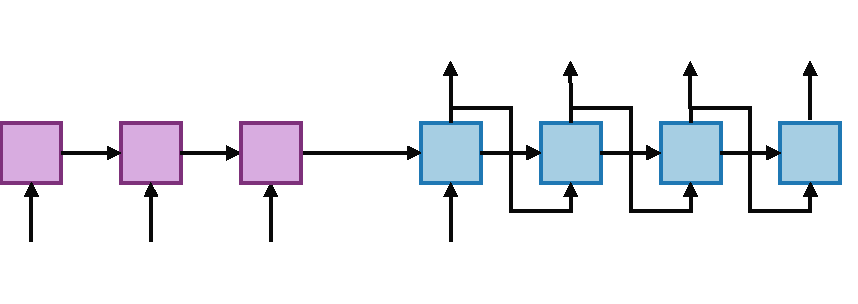
\includegraphics[width=1.0\textwidth]{imgs/seq2seq.pdf}
%   \caption{The sequence-to-sequence model}
%   \label{seq2seq}
% \end{figure}


\begin{figure}[htp]
  \centering
  \begin{overpic}[width=1.0\textwidth,tics=10]{imgs/seq2seq.pdf}
    \put (2.5,5) {\large$x_1$}
    \put (16.5,5) {\large$x_2$}
    \put (30.5,5) {\large$x_3$}
    \put (40,18.5) {\large$z$}
    \put (49,5) {\textit{START}}
    \put (51,29) {\large$y_1$}
    \put (65,29) {\large$y_2$}
    \put (79,29) {\large$y_3$}
    \put (93,29) {\large$y_4$}
  \end{overpic}
  \caption{The sequence-to-sequence model (unrolled)}
  \label{seq2seq}
\end{figure}


This model is trained as an autoencoder with the objective of minimising the mean squared error between the word embeddings of the input and output sequences. Because the latent space $z$ is of a significantly smaller dimension than the input space, the model is encouraged to encode the most salient features of the text in its latent embedding. Sampling around a point in the latent space should then ideally lead to decoded sentences that are semantically similar. This process is unfortunately not so simple, with previous work in applications of autoencoders to text finding that due to its discrete nature, the learned embedding space is rarely smooth and interpolation often results in poor-quality sentences \cite{cont}.

 To combat this issue, the final model (Fig.\ \ref{aae}) is modified to act as a variational autoencoder \cite{vae}, replacing the deterministic encoder with one that specifies the parameters of a diagonal gaussian distribution over $z$, encouraging the encoder to cover larger, smoother regions of the latent space. The posterior distribution is additionally constrained to follow a unit gaussian, preventing the encoder from simply encoding `discrete' points as distributions with a very small variance. This is achieved through adversarial training with the inclusion of a Wasserstein critic trained to estimate the probability $p(g)$ that a given $z$ is a sample from the encoder rather than a unit gaussian \cite{wgan}. While this constraint would typically be enforced by the inclusion of a loss term using the KL divergence, recent research argues that adversarial training can offer stronger gradient signals \cite{aae} and indeed, a recent survey of autoencoder-based text generation models found that samples from an adversarial autoencoder were typically more semantically similar to their input than the corresponding samples from a VAE \cite{evalall}.

\begin{figure}[htp!]
  \vspace{4mm}
  \centering
  \begin{overpic}[width=1.0\textwidth,tics=10]{imgs/aae.pdf}
    \put (6,25.5) {\large$\mathbf{x}$}
    \put (42,30) {\large$\mu$}
    \put (42,21) {\large$\sigma$}
    \put (35,4.5) {\large$z \sim \mathcal{N}(0,1)$}
    \put (49.5,27.5) {\large$z \sim \mathcal{N}(\mu,\sigma)$}
    \put (92,25.5) {\large$\mathbf{y}$}
    \put (90,6.5) {\large$\mathit{p}(g)$}
    \put (21,25.5) { encoder}
    \put (69,25.5) { decoder}
    \put (67.25,6.5) {\small discriminator}
  \end{overpic}
  \caption{The Adversarial Autoencoder model}
  \label{aae}
\end{figure}
% This model was trained using the adam optimiser with batch size 64 and learning rate 0.001. Following the suggestion of my boy, samples were augmented by replacing a word for the UNK token with a probability of 25\%. Each 



 % While this constraint is traditionally enforced by a loss term consisting of the KL divergence between the encoder distribution and a unit gaussian, recent research argues that better convergence can be achieved via adversarial training. 
% Taking inspiration from current machine translation models, the paraphrasing task is modelled as a problem of sequence-to-sequence learning


% \noindent The majority of current approaches to conditional language generation follow the structure of the sequence-to-sequence models popularised in machine translation \cite{seq2seq}. In such models, a recurrent neural network takes a variable-length sequence of tokens $x_1..x_t$ as an input and within its hidden state, encodes the sequence into fixed-length representation, effectively learning a conditional distribution over a latent space $p(z|x_1..x_t)$. An autoregressive decoder then takes this latent vector and predicts the next token in the output sequence $p(x_t | z, x_1.. x-{t-1}$



% neural network is used to encode the input sequence into a fixed-length latent vector, which is then used as input to an autoregressive decoder network to predict the next token in the output sequence.


% One possible approach to paraphrase generation is to learn a latent representation of the text and then 

% https://arxiv.org/pdf/1804.07972.pdf suggests aaee better


  % Diagram
  % Generating Sentences from a Continuous Space
  %   word dropout
  % Iain goodfellow aae paper
  %   regular gan is equiv to minimising kl divergence
  %     crappy gradients
  %   use wgan-gp instead
  %   nice wgan diagram from paper

  % posterior collapse = when the decoder ignores the latent code entirely
  % annealing

\subsection{Transfer Learning Autoencoder}

\noindent A potential flaw with the AAE model is that the reconstruction task is used as a surrogate for the true goal of finding a semantic embedding for text. While learning a semantic embedding would indeed be a sensible solution to the task, it is not guaranteed that this will be the solution that the model converges to. This issue can be resolved by making use of the ubiquity of sequence-to-sequence models in NLP to learn a more robust embedding via multi-task learning. Subramanian et al.\ (2018)\nocite{transfer} provide such a model, training a single encoder against multiple decoders, each given a unique task from machine translation, to natural language inference and constituency parsing. 

To repurpose this model for lexical steganography, the pre-trained sentence encoder can be used to train a decoder on the reconstruction task, with the encoder weights frozen in order to preserve their high-quality embeddings. Unlike the AAE model, this encoder is deterministic and the shape of the latent space is unknown. This means that extra care must be taken to ensure that interpolated points remain on the manifold. Subramanian et al.\ \citeyear{outlines} propose an approach for interpolating between two sentences $\mathbf{x}_1$ and $\mathbf{x}_2$ using the gradient signals from the decoder (Fig.\ \ref{manifold}). Starting from the latent embedding of $\mathbf{x}_1$, the current position in the latent space $h$ is updated in fixed steps of length $\alpha$ in accordance to Equation 4, and then passed to the decoder to generate a new interpolated sentence $q$.

\begin{equation}
  h' = h + \alpha\nabla_{h}\log\mathit{P}(\mathbf{x}_2|h)
\end{equation}

\begin{figure}[htp]
  \vspace{-4mm}
  \centering
  \begin{subfigure}[t]{0.49\textwidth}
    \begin{overpic}[width=0.9\textwidth,tics=10]{imgs/manifold1.pdf}
      \put (13, 68.5) {\large$\mathbf{x}_1$}
      \put (80, 42) {\large$\mathbf{x}_2$}
      \put (33, 61.5) {\large$y_1$}
      \put (56, 52.5) {\large$y_2$}
    \end{overpic}
  \caption{}
  \end{subfigure}
  \hfill
  \begin{subfigure}[t]{0.49\textwidth}
    \begin{overpic}[width=0.9\textwidth,tics=10]{imgs/manifold2.pdf}
      \put (13, 68.5) {\large$\mathbf{x}_1$}
      \put (80, 42) {\large$\mathbf{x}_2$}
      \put (27, 52.5) {\large$y_1$}
      \put (34, 34.5) {\large$y_2$}
      \put (40, 18.5) {\large$y_3$}
      \put (52, 20.5) {\large$y_4$}
      \put (62, 34.5) {\large$y_5$}
    \end{overpic}
  \caption{}
  \end{subfigure}
  \caption{Illustrations of linear interpolation (a) and gradient-based interpolation (b)}
  \label{manifold}
\end{figure}

\subsubsection{Multi-Path Interpolation}
In order to interpolate around the embedding of a given text $t$, we explore two modifications to the scheme provided. The Multi-Path approach (Algorithm \ref{multipath}) simply chooses a random point on the manifold $r$ and performs gradient-based interpolation between $r$ and $t$, repeating the process until enough unique texts are found. To ensure that all returned texts are suitably similar to $p$, a decoded text is only accepted if its BLEU score with relation to $p$ is greater than 0.2.\\

\vspace{-1mm}
 \begin{algorithm}[H]
    \SetAlgoLined
    \KwData{$t, n, \alpha$}
    \KwResult{Set $\mathrm{Q}$ consisting of $n$ paraphrases of the text $t$} 
    $\mathrm{Q} \gets \varnothing$\;
    $r \gets$ a randomly selected point on the manifold\;
    $h \gets \mathrm{encode}(r)$\;
    \While{$|\mathrm{Q}| > n$}{
      $h \gets h + \alpha\nabla_{h}\log\mathit{P}(t|h)$\;
      $q \gets \mathrm{decode}(h)$\;
      \If{$\textnormal{BLEU}(q, t) < 0.2$}{
          $\mathrm{Q} \gets \mathrm{Q} \cup \{q\}$\;
          \If{$q == t$}{
            $r \gets$ a randomly selected point on the manifold\;
            $h \gets \mathrm{encode}(r)$\;
        }
      }
    }
    \Return $\mathrm{Q}$\;   
    \caption{Multi-Path Interpolation (Forward)}
    \label{multipath}
\end{algorithm}

\subsubsection{Wandering Interpolation}
\noindent A possible issue with the multi-path approach is that depending on the randomly selected point, the algorithm may spend a large amount of time in distant areas of the manifold that are unlikely to decode to similar texts. The Wandering Interpolation scheme (Algorithm \ref{wander}) aims to solve this issue by constraining the exploration to latent vectors close to $t$. This is achieved by starting from $t$ and at each step, choosing a new target $r$ that is equal to $t$ with probabilty $p$ and otherwise, a randomly chosen point on the manifold. The value of $p$ can then be manually tuned to reach a suitable balance between exploring the latent space and staying in the vicinity of $t$.\\

\vspace{-1mm}
 \begin{algorithm}[H]
    \SetAlgoLined
    \KwData{$t, n, \alpha, p$}
    \KwResult{Set $\mathrm{Q}$ consisting of $n$ paraphrases of the text $t$} 
    $\mathrm{Q} \gets \varnothing$\;
    $h \gets \mathrm{encode}(t)$\;
    \While{$|\mathrm{Q}| > n$}{
      $r \gets t$ with probability $p$, else a randomly selected point on the manifold\;
      $h \gets h + \alpha\nabla_{h}\log\mathit{P}(r|h)$\;
      $q \gets \mathrm{decode}(h)$\;
      \If{$\textnormal{BLEU}(q, t) < 0.2$}{
          $\mathrm{Q} \gets \mathrm{Q} \cup \{q\}$\;
      }
    }
    \Return $\mathrm{Q}$\;   
    \caption{Wandering Interpolation}
    \label{wander}
\end{algorithm}

\subsubsection{Analogical Interpolation}
\noindent An alternative method can be devised for analogical interpolation by performing vector arithmetic on a set of known paraphrase pairs. Previous work has shown that for word embeddings, a surprisingly robust set of analogies of the form ``$x$ is to $y$ as $z$ is to ?'' can be computed through simple combinations of vectors \cite{queen}. For instance, taking the vector difference of the word embeddings for `paris' and `france' has been shown to yield a vector relating to the concept of a capital city, such that when added to the embedding of `warsaw', a vector close to the embedding of `poland' is obtained. Following the same process, a small set of sentences and their associated paraphrases can be used to create a set of vectors $\mathbf{p}$ in the latent space that correspond to the concept of paraphrasing. Interpolations around a particular sentence can then be generated by applying these paraphrase vectors to the embedded sentence (Fig.\ \ref{analogy}) and decoding the output.

% figure

\begin{figure}[htp]
  \centering
  \begin{subfigure}[t]{0.49\textwidth}
    \begin{overpic}[width=0.9\textwidth,tics=10]{imgs/analogy1.pdf}
      \put (66, 15) {\large$\mathbf{p}_3$}
      \put (47, 32) {\large$\mathbf{p}_2$}
      \put (35, 49) {\large$\mathbf{p}_1$}
    \end{overpic}
  \caption{}
  \end{subfigure}
  \hfill
  \begin{subfigure}[t]{0.49\textwidth}
    \begin{overpic}[width=0.9\textwidth,tics=10]{imgs/analogy2.pdf}
      \put (52, 24) {\large$\mathbf{x}_1$}
      \put (37, 38) {\large$\mathbf{p}_1$}
      \put (39, 22) {\large$\mathbf{p}_2$}
      \put (55.5, 33) {\large$\mathbf{p}_3$}
      \put (18, 40.5) {\large$y_1$}
      \put (17.5, 18) {\large$y_2$}
      \put (62, 50) {\large$y_3$}
    \end{overpic}
  \caption{}
  \end{subfigure}
  \caption{Illustration of the analogical interpolation scheme}
  \label{analogy}
\end{figure}


% This multi-task encoder is used to 

%  could then be used to train a decoder for the task of reconstruction as before, but with the encoder weights frozen so as to keep these robust embeddings at the expense of the latent space no longer being constrained to a gaussian, and with no immediate method to sample around a point. x propose a method for interpolating \textit{between} points by using the gradient. This could be modified to sdkfns;dfnasd

% therefore propose a model with a single encoder and multiple decoders, each with their own NLP task. 

%  that a more robust embedding could be found by jointly training a single encoder on a number of different NLP tasks, making use of the huge amount of research and data that has been collected, as well as providing a greater variety of gradient signals in order to prevent overfitting to a particular task. 

% As described in x, the transfer learned encoder could then be used to train a decoder for the task of reconstruction as before, but with the encoder weights frozen so as to keep these robust embeddings at the expense of the latent space no longer being constrained to a gaussian, and with no immediate method to sample around a point. x propose a method for interpolating \textit{between} points by using the gradient. This could be modified to sdkfns;dfnasd

% alternatively, a pahrasfsdf




% Another promising approach is to make use of the ubiquity of sequence-to-sequence models across the field of NLP. Intuitively, 



% Gaussian prior is potentially an issue - text is not fucking gaussian
% instead, let the latent code be whatever it needs to be and sample directly from it. 

% As discussed previously, naive interpolation is likely to go off manifold and return garbage.
% This alternative model aims to remedy this issue 

% sample directly from vae
% inverse sampling
% vector arithmetic
% gradient based

\subsection{Conditioning GPT2}

\noindent To extend the idea of repurposing existing models further, we investigate a method for conditioning the GPT2 model \cite{gpt2}, such that it is encouraged to output paraphrases of a given sentence. GPT2 differs substantially from the previously discussed models, using a powerful multi-headed self-attention mechanism to capture the internal dependencies of the input sequence. The encoder-decoder architecture is replaced by a decoder-transformer (Fig.\ \ref{gptb}) which models the input $\mathbf{x}$ and output $\mathbf{y}$ as a single combined sentence $\mathbf{m} = (x_1,\dots,x_T, \delta, y_1,\dots,y_{T'})$ where $\delta$ is a special delimiter character \cite{transdec}. The model is trained to maximise the likelihood of these combined sentences with the standard objective function, modified to operate within a context window of length $k$.
\begin{equation}
  \mathcal{L} = \sum_i\log \mathit{P}(m_i | m_{i-k}, \dots , m_{i-1}; \Theta)
\end{equation}
This ability to in some sense encode the problem definition within the input allows for the model to be easily trained on a wide range of tasks with minimal additional resources required, in comparison to the multi-task sequence-to-sequence model that required a separate decoder for each task. Along with the higher levels of parallelisation available from its lack of recurrent elements, this allows the model to be scaled up significantly, with Radford et al.\ training a model with 1.5B parameters on a corpus of text measuring 40GB. GPT2 has been shown to generalise spectacularly well to tasks within NLP, with a zero-shot performance on the question answering task exceeding that of 3 out of 4 baseline models \cite{gpt2}.

We therefore propose a scheme for constructing an input to GPT2 that implicitly encodes the task of paraphrasing. As shown in Fig.\ \ref{cond}, the model is supplied with a sequence of carefully delimited paraphrase pairs $\mathbf{m}_{cond}$ followed by $\mathbf{x}$. If GPT2 has in fact generalised well to language modelling then it will infer from this input pattern that a likely continuation of the input would be a paraphrase of $\mathbf{x}$. Additional paraphrases can then be generated by conditioning on an $\mathbf{m}_{cond}$ consisting of different paraphrase pairs.

\begin{figure}[htp]
\centering
\begin{minipage}[b]{.5\textwidth}
  \centering
  \begin{overpic}[width=0.7\textwidth,tics=10]{imgs/transformer.pdf}
    \put (15.5, 3.5) {Input Embedding}
    \put (18.5, 21.5) {Self-Attention}
    \put (21, 40) {Layer Norm}
    \put (21, 76) {Layer Norm}
    \put (3, 49) {12$\times$}
    \put (19, 58) {Feed Forward}
    \put (18, 93) {Text Prediction}
  \end{overpic}
  \captionof{figure}{The GPT2 model}
\label{gptb}
\end{minipage}%{}
\hfill
\begin{minipage}[b]{.5\textwidth}
  \centering
  \begin{tabular}{l}
\textit{He's choking me.} \\
\textit{he's strangling me.} \\
--- \\
\textit{Ben wore the palatinate gown.} \\
\textit{Ben wore the purple robe.} \\
--- \\
\textit{Whoa.} \\
\textit{stop right there.} \\
--- \\
\textit{Having my lunch!} \\
\textit{at lunch! } \\
--- \\
\textit{Hello, Pearly.} \\
\textit{hello, Pearly.} \\
--- \\
\textit{It was a lovely day.} \\
  \end{tabular}
  \captionof{figure}{Example input for paraphrasing ``It was a lovely day.''}
  \label{cond}
\begin{tikzpicture}[overlay, remember picture, yshift=.25\baselineskip, shorten >=.5pt, shorten <=.5pt]
\draw [decorate,decoration={brace,amplitude=10pt},xshift=-4pt,yshift=0pt,line width=0.4mm]
(-2.8,2.25) -- (-2.8,9.75) node [black,midway,xshift=-1cm,yshift=0.5mm] 
{\large$\mathbf{m}_{cond}$};
    \put (-92, 54) {\large$\mathbf{x}$}
  \end{tikzpicture}
\vspace{-8.6mm}
\end{minipage}
\end{figure}

% \subsection{Training}
\vspace{2mm}
\section{Results}

\noindent Evaluation was performed using the P{\footnotesize ARA}NMT corpus, a set of 50M paraphrase pairs with an associated `paraphrase score' to denote the extent of semantic equivalence between each pair \cite{paranmt}. The paraphrase pairs were generated using a corpus of translations from English to Czech, with each pair consisting of the original English sentence and the associated Czech sentence translated into English via an NMT model.
% \subsection{Latent Space Exploration}
% interpolation around aaee

% Reconstruction loss
\subsection{Capacity}

\noindent We first investigate the steganographic capacity of each approach. This is achieved by plotting the textual similarity between each system's output and the 10,000 highest scoring paraphrase pairs in P{\footnotesize ARA}NMT, with the understanding that a system's steganographic capacity is the highest number of encoded payload bits at which the returned stegotexts are both fluent and semantically similar to the cover text. Since fluency cannot be automatically quantified, our estimations are based only on the relevance of the stegotext with respect to the cover text, measured as the BLEU-2 score between the stegotext and both the original sentence and its paraphrase in P{\footnotesize ARA}NMT, with fluency later measured in a user study. Relevance measures are taken for each model, set to encode random payloads of lengths in the range of 1 to 4 bits. 


\begin{figure}[htp]
  \centering
  % Created by tikzDevice version 0.12 on 2019-04-30 12:38:12
% !TEX encoding = UTF-8 Unicode
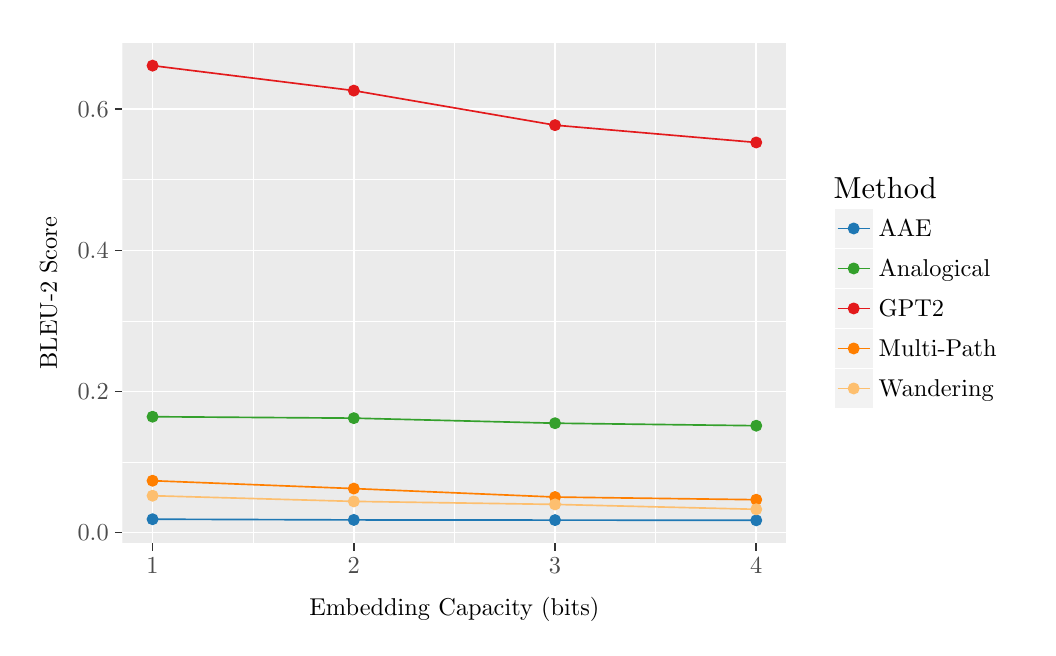
\begin{tikzpicture}[x=1pt,y=1pt]
\definecolor{fillColor}{RGB}{255,255,255}
\path[use as bounding box,fill=fillColor,fill opacity=0.00] (0,0) rectangle (361.35,216.81);
\begin{scope}
\path[clip] (  0.00,  0.00) rectangle (361.35,216.81);
\definecolor{drawColor}{RGB}{255,255,255}
\definecolor{fillColor}{RGB}{255,255,255}

\path[draw=drawColor,line width= 0.6pt,line join=round,line cap=round,fill=fillColor] (  0.00,  0.00) rectangle (361.35,216.81);
\end{scope}
\begin{scope}
\path[clip] ( 34.22, 30.57) rectangle (274.18,211.31);
\definecolor{fillColor}{gray}{0.92}

\path[fill=fillColor] ( 34.22, 30.57) rectangle (274.18,211.31);
\definecolor{drawColor}{RGB}{255,255,255}

\path[draw=drawColor,line width= 0.3pt,line join=round] ( 34.22, 59.86) --
	(274.18, 59.86);

\path[draw=drawColor,line width= 0.3pt,line join=round] ( 34.22,110.84) --
	(274.18,110.84);

\path[draw=drawColor,line width= 0.3pt,line join=round] ( 34.22,161.82) --
	(274.18,161.82);

\path[draw=drawColor,line width= 0.3pt,line join=round] ( 81.49, 30.57) --
	( 81.49,211.31);

\path[draw=drawColor,line width= 0.3pt,line join=round] (154.20, 30.57) --
	(154.20,211.31);

\path[draw=drawColor,line width= 0.3pt,line join=round] (226.92, 30.57) --
	(226.92,211.31);

\path[draw=drawColor,line width= 0.6pt,line join=round] ( 34.22, 34.36) --
	(274.18, 34.36);

\path[draw=drawColor,line width= 0.6pt,line join=round] ( 34.22, 85.35) --
	(274.18, 85.35);

\path[draw=drawColor,line width= 0.6pt,line join=round] ( 34.22,136.33) --
	(274.18,136.33);

\path[draw=drawColor,line width= 0.6pt,line join=round] ( 34.22,187.32) --
	(274.18,187.32);

\path[draw=drawColor,line width= 0.6pt,line join=round] ( 45.13, 30.57) --
	( 45.13,211.31);

\path[draw=drawColor,line width= 0.6pt,line join=round] (117.85, 30.57) --
	(117.85,211.31);

\path[draw=drawColor,line width= 0.6pt,line join=round] (190.56, 30.57) --
	(190.56,211.31);

\path[draw=drawColor,line width= 0.6pt,line join=round] (263.27, 30.57) --
	(263.27,211.31);
\definecolor{drawColor}{RGB}{31,120,180}

\path[draw=drawColor,line width= 0.6pt,line join=round] ( 45.13, 39.19) --
	(117.85, 38.94) --
	(190.56, 38.87) --
	(263.27, 38.79);
\definecolor{drawColor}{RGB}{52,160,44}

\path[draw=drawColor,line width= 0.6pt,line join=round] ( 45.13, 76.23) --
	(117.85, 75.71) --
	(190.56, 73.88) --
	(263.27, 72.98);
\definecolor{drawColor}{RGB}{227,26,28}

\path[draw=drawColor,line width= 0.6pt,line join=round] ( 45.13,203.09) --
	(117.85,194.07) --
	(190.56,181.58) --
	(263.27,175.33);
\definecolor{drawColor}{RGB}{255,127,0}

\path[draw=drawColor,line width= 0.6pt,line join=round] ( 45.13, 53.10) --
	(117.85, 50.26) --
	(190.56, 47.20) --
	(263.27, 46.24);
\definecolor{drawColor}{RGB}{253,191,111}

\path[draw=drawColor,line width= 0.6pt,line join=round] ( 45.13, 47.68) --
	(117.85, 45.63) --
	(190.56, 44.54) --
	(263.27, 42.77);
\definecolor{drawColor}{RGB}{31,120,180}
\definecolor{fillColor}{RGB}{31,120,180}

\path[draw=drawColor,line width= 0.4pt,line join=round,line cap=round,fill=fillColor] ( 45.13, 39.19) circle (  1.96);

\path[draw=drawColor,line width= 0.4pt,line join=round,line cap=round,fill=fillColor] (117.85, 38.94) circle (  1.96);

\path[draw=drawColor,line width= 0.4pt,line join=round,line cap=round,fill=fillColor] (190.56, 38.87) circle (  1.96);

\path[draw=drawColor,line width= 0.4pt,line join=round,line cap=round,fill=fillColor] (263.27, 38.79) circle (  1.96);
\definecolor{drawColor}{RGB}{227,26,28}
\definecolor{fillColor}{RGB}{227,26,28}

\path[draw=drawColor,line width= 0.4pt,line join=round,line cap=round,fill=fillColor] ( 45.13,203.09) circle (  1.96);

\path[draw=drawColor,line width= 0.4pt,line join=round,line cap=round,fill=fillColor] (117.85,194.07) circle (  1.96);

\path[draw=drawColor,line width= 0.4pt,line join=round,line cap=round,fill=fillColor] (190.56,181.58) circle (  1.96);

\path[draw=drawColor,line width= 0.4pt,line join=round,line cap=round,fill=fillColor] (263.27,175.33) circle (  1.96);
\definecolor{drawColor}{RGB}{255,127,0}
\definecolor{fillColor}{RGB}{255,127,0}

\path[draw=drawColor,line width= 0.4pt,line join=round,line cap=round,fill=fillColor] ( 45.13, 53.10) circle (  1.96);

\path[draw=drawColor,line width= 0.4pt,line join=round,line cap=round,fill=fillColor] (117.85, 50.26) circle (  1.96);

\path[draw=drawColor,line width= 0.4pt,line join=round,line cap=round,fill=fillColor] (190.56, 47.20) circle (  1.96);

\path[draw=drawColor,line width= 0.4pt,line join=round,line cap=round,fill=fillColor] (263.27, 46.24) circle (  1.96);
\definecolor{drawColor}{RGB}{52,160,44}
\definecolor{fillColor}{RGB}{52,160,44}

\path[draw=drawColor,line width= 0.4pt,line join=round,line cap=round,fill=fillColor] ( 45.13, 76.23) circle (  1.96);

\path[draw=drawColor,line width= 0.4pt,line join=round,line cap=round,fill=fillColor] (117.85, 75.71) circle (  1.96);

\path[draw=drawColor,line width= 0.4pt,line join=round,line cap=round,fill=fillColor] (190.56, 73.88) circle (  1.96);

\path[draw=drawColor,line width= 0.4pt,line join=round,line cap=round,fill=fillColor] (263.27, 72.98) circle (  1.96);
\definecolor{drawColor}{RGB}{253,191,111}
\definecolor{fillColor}{RGB}{253,191,111}

\path[draw=drawColor,line width= 0.4pt,line join=round,line cap=round,fill=fillColor] ( 45.13, 47.68) circle (  1.96);

\path[draw=drawColor,line width= 0.4pt,line join=round,line cap=round,fill=fillColor] (117.85, 45.63) circle (  1.96);

\path[draw=drawColor,line width= 0.4pt,line join=round,line cap=round,fill=fillColor] (190.56, 44.54) circle (  1.96);

\path[draw=drawColor,line width= 0.4pt,line join=round,line cap=round,fill=fillColor] (263.27, 42.77) circle (  1.96);
\end{scope}
\begin{scope}
\path[clip] (  0.00,  0.00) rectangle (361.35,216.81);
\definecolor{drawColor}{gray}{0.30}

\node[text=drawColor,anchor=base east,inner sep=0pt, outer sep=0pt, scale=  0.88] at ( 29.27, 31.33) {0.0};

\node[text=drawColor,anchor=base east,inner sep=0pt, outer sep=0pt, scale=  0.88] at ( 29.27, 82.32) {0.2};

\node[text=drawColor,anchor=base east,inner sep=0pt, outer sep=0pt, scale=  0.88] at ( 29.27,133.30) {0.4};

\node[text=drawColor,anchor=base east,inner sep=0pt, outer sep=0pt, scale=  0.88] at ( 29.27,184.29) {0.6};
\end{scope}
\begin{scope}
\path[clip] (  0.00,  0.00) rectangle (361.35,216.81);
\definecolor{drawColor}{gray}{0.20}

\path[draw=drawColor,line width= 0.6pt,line join=round] ( 31.47, 34.36) --
	( 34.22, 34.36);

\path[draw=drawColor,line width= 0.6pt,line join=round] ( 31.47, 85.35) --
	( 34.22, 85.35);

\path[draw=drawColor,line width= 0.6pt,line join=round] ( 31.47,136.33) --
	( 34.22,136.33);

\path[draw=drawColor,line width= 0.6pt,line join=round] ( 31.47,187.32) --
	( 34.22,187.32);
\end{scope}
\begin{scope}
\path[clip] (  0.00,  0.00) rectangle (361.35,216.81);
\definecolor{drawColor}{gray}{0.20}

\path[draw=drawColor,line width= 0.6pt,line join=round] ( 45.13, 27.82) --
	( 45.13, 30.57);

\path[draw=drawColor,line width= 0.6pt,line join=round] (117.85, 27.82) --
	(117.85, 30.57);

\path[draw=drawColor,line width= 0.6pt,line join=round] (190.56, 27.82) --
	(190.56, 30.57);

\path[draw=drawColor,line width= 0.6pt,line join=round] (263.27, 27.82) --
	(263.27, 30.57);
\end{scope}
\begin{scope}
\path[clip] (  0.00,  0.00) rectangle (361.35,216.81);
\definecolor{drawColor}{gray}{0.30}

\node[text=drawColor,anchor=base,inner sep=0pt, outer sep=0pt, scale=  0.88] at ( 45.13, 19.56) {1};

\node[text=drawColor,anchor=base,inner sep=0pt, outer sep=0pt, scale=  0.88] at (117.85, 19.56) {2};

\node[text=drawColor,anchor=base,inner sep=0pt, outer sep=0pt, scale=  0.88] at (190.56, 19.56) {3};

\node[text=drawColor,anchor=base,inner sep=0pt, outer sep=0pt, scale=  0.88] at (263.27, 19.56) {4};
\end{scope}
\begin{scope}
\path[clip] (  0.00,  0.00) rectangle (361.35,216.81);
\definecolor{drawColor}{RGB}{0,0,0}

\node[text=drawColor,anchor=base,inner sep=0pt, outer sep=0pt, scale=  0.88] at (154.20,  4.25) {Embedding Capacity (bits)};
\end{scope}
\begin{scope}
\path[clip] (  0.00,  0.00) rectangle (361.35,216.81);
\definecolor{drawColor}{RGB}{0,0,0}

\node[text=drawColor,rotate= 90.00,anchor=base,inner sep=0pt, outer sep=0pt, scale=  0.88] at ( 10.59,120.94) {BLEU-2 Score};
\end{scope}
\begin{scope}
\path[clip] (  0.00,  0.00) rectangle (361.35,216.81);
\definecolor{fillColor}{RGB}{255,255,255}

\path[fill=fillColor] (285.56, 73.52) rectangle (355.85,168.36);
\end{scope}
\begin{scope}
\path[clip] (  0.00,  0.00) rectangle (361.35,216.81);
\definecolor{drawColor}{RGB}{0,0,0}

\node[text=drawColor,anchor=base west,inner sep=0pt, outer sep=0pt, scale=  1.10] at (291.25,155.09) {Method};
\end{scope}
\begin{scope}
\path[clip] (  0.00,  0.00) rectangle (361.35,216.81);
\definecolor{drawColor}{RGB}{255,255,255}
\definecolor{fillColor}{gray}{0.95}

\path[draw=drawColor,line width= 0.6pt,line join=round,line cap=round,fill=fillColor] (291.25,137.03) rectangle (305.71,151.48);
\end{scope}
\begin{scope}
\path[clip] (  0.00,  0.00) rectangle (361.35,216.81);
\definecolor{drawColor}{RGB}{31,120,180}

\path[draw=drawColor,line width= 0.6pt,line join=round] (292.70,144.25) -- (304.26,144.25);
\end{scope}
\begin{scope}
\path[clip] (  0.00,  0.00) rectangle (361.35,216.81);
\definecolor{drawColor}{RGB}{31,120,180}
\definecolor{fillColor}{RGB}{31,120,180}

\path[draw=drawColor,line width= 0.4pt,line join=round,line cap=round,fill=fillColor] (298.48,144.25) circle (  1.96);
\end{scope}
\begin{scope}
\path[clip] (  0.00,  0.00) rectangle (361.35,216.81);
\definecolor{drawColor}{RGB}{255,255,255}
\definecolor{fillColor}{gray}{0.95}

\path[draw=drawColor,line width= 0.6pt,line join=round,line cap=round,fill=fillColor] (291.25,122.57) rectangle (305.71,137.03);
\end{scope}
\begin{scope}
\path[clip] (  0.00,  0.00) rectangle (361.35,216.81);
\definecolor{drawColor}{RGB}{52,160,44}

\path[draw=drawColor,line width= 0.6pt,line join=round] (292.70,129.80) -- (304.26,129.80);
\end{scope}
\begin{scope}
\path[clip] (  0.00,  0.00) rectangle (361.35,216.81);
\definecolor{drawColor}{RGB}{52,160,44}
\definecolor{fillColor}{RGB}{52,160,44}

\path[draw=drawColor,line width= 0.4pt,line join=round,line cap=round,fill=fillColor] (298.48,129.80) circle (  1.96);
\end{scope}
\begin{scope}
\path[clip] (  0.00,  0.00) rectangle (361.35,216.81);
\definecolor{drawColor}{RGB}{255,255,255}
\definecolor{fillColor}{gray}{0.95}

\path[draw=drawColor,line width= 0.6pt,line join=round,line cap=round,fill=fillColor] (291.25,108.12) rectangle (305.71,122.57);
\end{scope}
\begin{scope}
\path[clip] (  0.00,  0.00) rectangle (361.35,216.81);
\definecolor{drawColor}{RGB}{227,26,28}

\path[draw=drawColor,line width= 0.6pt,line join=round] (292.70,115.35) -- (304.26,115.35);
\end{scope}
\begin{scope}
\path[clip] (  0.00,  0.00) rectangle (361.35,216.81);
\definecolor{drawColor}{RGB}{227,26,28}
\definecolor{fillColor}{RGB}{227,26,28}

\path[draw=drawColor,line width= 0.4pt,line join=round,line cap=round,fill=fillColor] (298.48,115.35) circle (  1.96);
\end{scope}
\begin{scope}
\path[clip] (  0.00,  0.00) rectangle (361.35,216.81);
\definecolor{drawColor}{RGB}{255,255,255}
\definecolor{fillColor}{gray}{0.95}

\path[draw=drawColor,line width= 0.6pt,line join=round,line cap=round,fill=fillColor] (291.25, 93.66) rectangle (305.71,108.12);
\end{scope}
\begin{scope}
\path[clip] (  0.00,  0.00) rectangle (361.35,216.81);
\definecolor{drawColor}{RGB}{255,127,0}

\path[draw=drawColor,line width= 0.6pt,line join=round] (292.70,100.89) -- (304.26,100.89);
\end{scope}
\begin{scope}
\path[clip] (  0.00,  0.00) rectangle (361.35,216.81);
\definecolor{drawColor}{RGB}{255,127,0}
\definecolor{fillColor}{RGB}{255,127,0}

\path[draw=drawColor,line width= 0.4pt,line join=round,line cap=round,fill=fillColor] (298.48,100.89) circle (  1.96);
\end{scope}
\begin{scope}
\path[clip] (  0.00,  0.00) rectangle (361.35,216.81);
\definecolor{drawColor}{RGB}{255,255,255}
\definecolor{fillColor}{gray}{0.95}

\path[draw=drawColor,line width= 0.6pt,line join=round,line cap=round,fill=fillColor] (291.25, 79.21) rectangle (305.71, 93.66);
\end{scope}
\begin{scope}
\path[clip] (  0.00,  0.00) rectangle (361.35,216.81);
\definecolor{drawColor}{RGB}{253,191,111}

\path[draw=drawColor,line width= 0.6pt,line join=round] (292.70, 86.44) -- (304.26, 86.44);
\end{scope}
\begin{scope}
\path[clip] (  0.00,  0.00) rectangle (361.35,216.81);
\definecolor{drawColor}{RGB}{253,191,111}
\definecolor{fillColor}{RGB}{253,191,111}

\path[draw=drawColor,line width= 0.4pt,line join=round,line cap=round,fill=fillColor] (298.48, 86.44) circle (  1.96);
\end{scope}
\begin{scope}
\path[clip] (  0.00,  0.00) rectangle (361.35,216.81);
\definecolor{drawColor}{RGB}{0,0,0}

\node[text=drawColor,anchor=base west,inner sep=0pt, outer sep=0pt, scale=  0.88] at (307.51,141.22) {AAE};
\end{scope}
\begin{scope}
\path[clip] (  0.00,  0.00) rectangle (361.35,216.81);
\definecolor{drawColor}{RGB}{0,0,0}

\node[text=drawColor,anchor=base west,inner sep=0pt, outer sep=0pt, scale=  0.88] at (307.51,126.77) {Analogical};
\end{scope}
\begin{scope}
\path[clip] (  0.00,  0.00) rectangle (361.35,216.81);
\definecolor{drawColor}{RGB}{0,0,0}

\node[text=drawColor,anchor=base west,inner sep=0pt, outer sep=0pt, scale=  0.88] at (307.51,112.32) {GPT2};
\end{scope}
\begin{scope}
\path[clip] (  0.00,  0.00) rectangle (361.35,216.81);
\definecolor{drawColor}{RGB}{0,0,0}

\node[text=drawColor,anchor=base west,inner sep=0pt, outer sep=0pt, scale=  0.88] at (307.51, 97.86) {Multi-Path};
\end{scope}
\begin{scope}
\path[clip] (  0.00,  0.00) rectangle (361.35,216.81);
\definecolor{drawColor}{RGB}{0,0,0}

\node[text=drawColor,anchor=base west,inner sep=0pt, outer sep=0pt, scale=  0.88] at (307.51, 83.41) {Wandering};
\end{scope}
\end{tikzpicture}

  \caption{Mean output relevance over increasing embedding capacities}
  \label{capacity}
\end{figure}

\noindent  As shown in Fig. \ref{capacity}, the AAE model does not appear to generalise to unseen samples, receiving a very low BLEU score even for a capacity of one. Results are marginally improved in the transfer learning model, with the analogical interpolation scheme appearing to outperform the gradient-based approaches, although a BLEU score in the range of 0.1 to 0.2 is still relatively poor. Performance for GPT2 however, is noticeably better across the board, achieving BLEU scores of around 0.6 with only a minor deterioration as the capacity is increased. Providing the output for GPT2 is also fluent, this would indicate a capacity rivalling that of CoverTweet, the current leading lexical steganography system. 

% change in bleu over capacity (line graph)
% BLEU/ perplexity

% 1,2,4

% https://arxiv.org/pdf/1808.04444.pdf cool
\subsection{User Study}

\noindent In order to verify the results of the metric-based evaluation, and further investigate the quality of each system's output, a user study was performed using the method described by C\'ifka et al.\ \citeyear{evalall}. Twenty participants were supplied with a set of 25 samples from each model, set to encode with a capacity of four bits, along with the associated paraphrase sample from P{\footnotesize ARA}NMT. The participants were then instructed to score each sample on a 1-5 Likert scale for both the relevance of the output to the original sentence, and the overall fluency of the text, regardless of meaning. For the transfer learning model, we used the analogical interpolation scheme as it was the best performing method in the automatic evaluation.

\subsubsection{Relevance}

\noindent As shown in Fig.\ \ref{relevance}, the user evaluations for relevance support the initial metric-based evaluation, with the AAE model scoring very poorly, the transfer learning model offering a slight improvement, and GPT2 vastly outperforming both models with a mean relevance score of 3.93, compared to the mean P{\footnotesize ARA}NMT score of 4.64. A set of paired Student's t-tests were performed on these results (Table \ref{relevancetable}), indicating with a high level of confidence that the samples from GPT2 are of a higher relevance on average than both the AAE and transfer learning models, but less relevant than samples from P{\footnotesize ARA}NMT.

\begin{figure}[htp]
  \centering
  % Created by tikzDevice version 0.12 on 2019-04-30 13:25:14
% !TEX encoding = UTF-8 Unicode
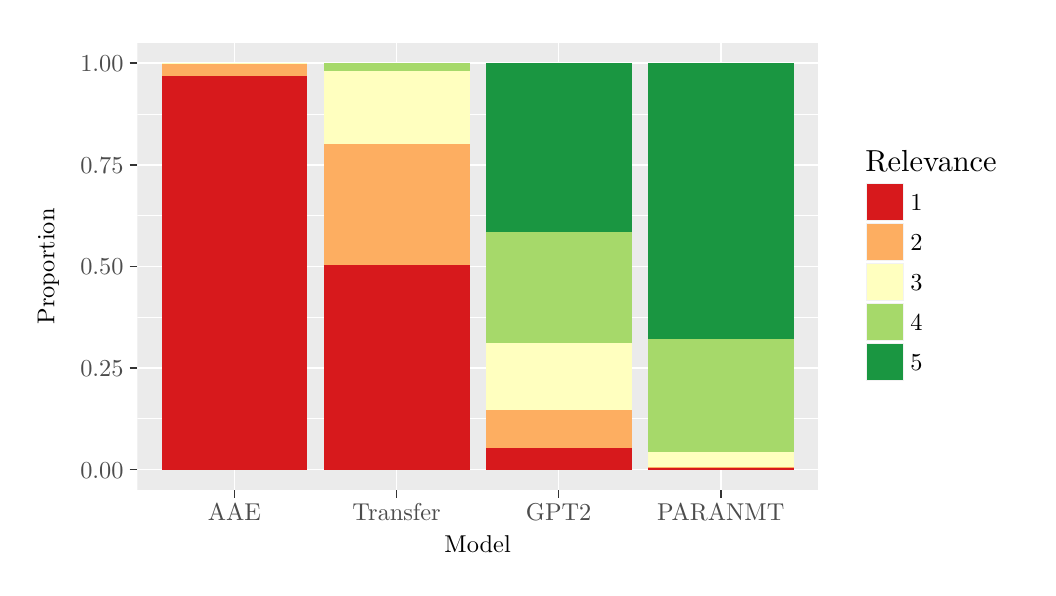
\begin{tikzpicture}[x=1pt,y=1pt]
\definecolor{fillColor}{RGB}{255,255,255}
\path[use as bounding box,fill=fillColor,fill opacity=0.00] (0,0) rectangle (361.35,195.13);
\begin{scope}
\path[clip] (  0.00,  0.00) rectangle (361.35,195.13);
\definecolor{drawColor}{RGB}{255,255,255}
\definecolor{fillColor}{RGB}{255,255,255}

\path[draw=drawColor,line width= 0.6pt,line join=round,line cap=round,fill=fillColor] (  0.00,  0.00) rectangle (361.35,195.13);
\end{scope}
\begin{scope}
\path[clip] ( 39.60, 28.07) rectangle (285.59,189.63);
\definecolor{fillColor}{gray}{0.92}

\path[fill=fillColor] ( 39.60, 28.07) rectangle (285.59,189.63);
\definecolor{drawColor}{RGB}{255,255,255}

\path[draw=drawColor,line width= 0.3pt,line join=round] ( 39.60, 53.77) --
	(285.59, 53.77);

\path[draw=drawColor,line width= 0.3pt,line join=round] ( 39.60, 90.49) --
	(285.59, 90.49);

\path[draw=drawColor,line width= 0.3pt,line join=round] ( 39.60,127.21) --
	(285.59,127.21);

\path[draw=drawColor,line width= 0.3pt,line join=round] ( 39.60,163.93) --
	(285.59,163.93);

\path[draw=drawColor,line width= 0.6pt,line join=round] ( 39.60, 35.42) --
	(285.59, 35.42);

\path[draw=drawColor,line width= 0.6pt,line join=round] ( 39.60, 72.13) --
	(285.59, 72.13);

\path[draw=drawColor,line width= 0.6pt,line join=round] ( 39.60,108.85) --
	(285.59,108.85);

\path[draw=drawColor,line width= 0.6pt,line join=round] ( 39.60,145.57) --
	(285.59,145.57);

\path[draw=drawColor,line width= 0.6pt,line join=round] ( 39.60,182.29) --
	(285.59,182.29);

\path[draw=drawColor,line width= 0.6pt,line join=round] ( 74.74, 28.07) --
	( 74.74,189.63);

\path[draw=drawColor,line width= 0.6pt,line join=round] (133.31, 28.07) --
	(133.31,189.63);

\path[draw=drawColor,line width= 0.6pt,line join=round] (191.87, 28.07) --
	(191.87,189.63);

\path[draw=drawColor,line width= 0.6pt,line join=round] (250.44, 28.07) --
	(250.44,189.63);
\definecolor{fillColor}{RGB}{215,25,28}

\path[fill=fillColor] ( 48.38, 35.42) rectangle (101.09,177.84);
\definecolor{fillColor}{RGB}{253,174,97}

\path[fill=fillColor] ( 48.38,177.84) rectangle (101.09,181.99);
\definecolor{fillColor}{RGB}{255,255,191}

\path[fill=fillColor] ( 48.38,181.99) rectangle (101.09,182.29);
\definecolor{fillColor}{RGB}{215,25,28}

\path[fill=fillColor] (106.95, 35.42) rectangle (159.66,109.44);
\definecolor{fillColor}{RGB}{253,174,97}

\path[fill=fillColor] (106.95,109.44) rectangle (159.66,152.97);
\definecolor{fillColor}{RGB}{255,255,191}

\path[fill=fillColor] (106.95,152.97) rectangle (159.66,179.62);
\definecolor{fillColor}{RGB}{166,217,106}

\path[fill=fillColor] (106.95,179.62) rectangle (159.66,182.29);
\definecolor{fillColor}{RGB}{215,25,28}

\path[fill=fillColor] (165.52, 35.42) rectangle (218.23, 43.11);
\definecolor{fillColor}{RGB}{253,174,97}

\path[fill=fillColor] (165.52, 43.11) rectangle (218.23, 57.03);
\definecolor{fillColor}{RGB}{255,255,191}

\path[fill=fillColor] (165.52, 57.03) rectangle (218.23, 81.02);
\definecolor{fillColor}{RGB}{166,217,106}

\path[fill=fillColor] (165.52, 81.02) rectangle (218.23,121.29);
\definecolor{fillColor}{RGB}{26,150,65}

\path[fill=fillColor] (165.52,121.29) rectangle (218.23,182.29);
\definecolor{fillColor}{RGB}{215,25,28}

\path[fill=fillColor] (224.09, 35.42) rectangle (276.80, 36.01);
\definecolor{fillColor}{RGB}{253,174,97}

\path[fill=fillColor] (224.09, 36.01) rectangle (276.80, 36.30);
\definecolor{fillColor}{RGB}{255,255,191}

\path[fill=fillColor] (224.09, 36.30) rectangle (276.80, 41.93);
\definecolor{fillColor}{RGB}{166,217,106}

\path[fill=fillColor] (224.09, 41.93) rectangle (276.80, 82.79);
\definecolor{fillColor}{RGB}{26,150,65}

\path[fill=fillColor] (224.09, 82.79) rectangle (276.80,182.29);
\end{scope}
\begin{scope}
\path[clip] (  0.00,  0.00) rectangle (361.35,195.13);
\definecolor{drawColor}{gray}{0.30}

\node[text=drawColor,anchor=base east,inner sep=0pt, outer sep=0pt, scale=  0.88] at ( 34.65, 32.38) {0.00};

\node[text=drawColor,anchor=base east,inner sep=0pt, outer sep=0pt, scale=  0.88] at ( 34.65, 69.10) {0.25};

\node[text=drawColor,anchor=base east,inner sep=0pt, outer sep=0pt, scale=  0.88] at ( 34.65,105.82) {0.50};

\node[text=drawColor,anchor=base east,inner sep=0pt, outer sep=0pt, scale=  0.88] at ( 34.65,142.54) {0.75};

\node[text=drawColor,anchor=base east,inner sep=0pt, outer sep=0pt, scale=  0.88] at ( 34.65,179.26) {1.00};
\end{scope}
\begin{scope}
\path[clip] (  0.00,  0.00) rectangle (361.35,195.13);
\definecolor{drawColor}{gray}{0.20}

\path[draw=drawColor,line width= 0.6pt,line join=round] ( 36.85, 35.42) --
	( 39.60, 35.42);

\path[draw=drawColor,line width= 0.6pt,line join=round] ( 36.85, 72.13) --
	( 39.60, 72.13);

\path[draw=drawColor,line width= 0.6pt,line join=round] ( 36.85,108.85) --
	( 39.60,108.85);

\path[draw=drawColor,line width= 0.6pt,line join=round] ( 36.85,145.57) --
	( 39.60,145.57);

\path[draw=drawColor,line width= 0.6pt,line join=round] ( 36.85,182.29) --
	( 39.60,182.29);
\end{scope}
\begin{scope}
\path[clip] (  0.00,  0.00) rectangle (361.35,195.13);
\definecolor{drawColor}{gray}{0.20}

\path[draw=drawColor,line width= 0.6pt,line join=round] ( 74.74, 25.32) --
	( 74.74, 28.07);

\path[draw=drawColor,line width= 0.6pt,line join=round] (133.31, 25.32) --
	(133.31, 28.07);

\path[draw=drawColor,line width= 0.6pt,line join=round] (191.87, 25.32) --
	(191.87, 28.07);

\path[draw=drawColor,line width= 0.6pt,line join=round] (250.44, 25.32) --
	(250.44, 28.07);
\end{scope}
\begin{scope}
\path[clip] (  0.00,  0.00) rectangle (361.35,195.13);
\definecolor{drawColor}{gray}{0.30}

\node[text=drawColor,anchor=base,inner sep=0pt, outer sep=0pt, scale=  0.88] at ( 74.74, 17.06) {AAE};

\node[text=drawColor,anchor=base,inner sep=0pt, outer sep=0pt, scale=  0.88] at (133.31, 17.06) {Transfer};

\node[text=drawColor,anchor=base,inner sep=0pt, outer sep=0pt, scale=  0.88] at (191.87, 17.06) {GPT2};

\node[text=drawColor,anchor=base,inner sep=0pt, outer sep=0pt, scale=  0.88] at (250.44, 17.06) {PARANMT};
\end{scope}
\begin{scope}
\path[clip] (  0.00,  0.00) rectangle (361.35,195.13);
\definecolor{drawColor}{RGB}{0,0,0}

\node[text=drawColor,anchor=base,inner sep=0pt, outer sep=0pt, scale=  0.88] at (162.59,  5.50) {Model};
\end{scope}
\begin{scope}
\path[clip] (  0.00,  0.00) rectangle (361.35,195.13);
\definecolor{drawColor}{RGB}{0,0,0}

\node[text=drawColor,rotate= 90.00,anchor=base,inner sep=0pt, outer sep=0pt, scale=  0.88] at (  9.62,108.85) {Proportion};
\end{scope}
\begin{scope}
\path[clip] (  0.00,  0.00) rectangle (361.35,195.13);
\definecolor{fillColor}{RGB}{255,255,255}

\path[fill=fillColor] (296.97, 61.43) rectangle (355.85,156.27);
\end{scope}
\begin{scope}
\path[clip] (  0.00,  0.00) rectangle (361.35,195.13);
\definecolor{drawColor}{RGB}{0,0,0}

\node[text=drawColor,anchor=base west,inner sep=0pt, outer sep=0pt, scale=  1.10] at (302.66,143.00) {Relevance};
\end{scope}
\begin{scope}
\path[clip] (  0.00,  0.00) rectangle (361.35,195.13);
\definecolor{drawColor}{RGB}{255,255,255}
\definecolor{fillColor}{gray}{0.95}

\path[draw=drawColor,line width= 0.6pt,line join=round,line cap=round,fill=fillColor] (302.66,124.94) rectangle (317.11,139.39);
\end{scope}
\begin{scope}
\path[clip] (  0.00,  0.00) rectangle (361.35,195.13);
\definecolor{fillColor}{RGB}{215,25,28}

\path[fill=fillColor] (303.37,125.65) rectangle (316.40,138.68);
\end{scope}
\begin{scope}
\path[clip] (  0.00,  0.00) rectangle (361.35,195.13);
\definecolor{drawColor}{RGB}{255,255,255}
\definecolor{fillColor}{gray}{0.95}

\path[draw=drawColor,line width= 0.6pt,line join=round,line cap=round,fill=fillColor] (302.66,110.48) rectangle (317.11,124.94);
\end{scope}
\begin{scope}
\path[clip] (  0.00,  0.00) rectangle (361.35,195.13);
\definecolor{fillColor}{RGB}{253,174,97}

\path[fill=fillColor] (303.37,111.19) rectangle (316.40,124.23);
\end{scope}
\begin{scope}
\path[clip] (  0.00,  0.00) rectangle (361.35,195.13);
\definecolor{drawColor}{RGB}{255,255,255}
\definecolor{fillColor}{gray}{0.95}

\path[draw=drawColor,line width= 0.6pt,line join=round,line cap=round,fill=fillColor] (302.66, 96.03) rectangle (317.11,110.48);
\end{scope}
\begin{scope}
\path[clip] (  0.00,  0.00) rectangle (361.35,195.13);
\definecolor{fillColor}{RGB}{255,255,191}

\path[fill=fillColor] (303.37, 96.74) rectangle (316.40,109.77);
\end{scope}
\begin{scope}
\path[clip] (  0.00,  0.00) rectangle (361.35,195.13);
\definecolor{drawColor}{RGB}{255,255,255}
\definecolor{fillColor}{gray}{0.95}

\path[draw=drawColor,line width= 0.6pt,line join=round,line cap=round,fill=fillColor] (302.66, 81.57) rectangle (317.11, 96.03);
\end{scope}
\begin{scope}
\path[clip] (  0.00,  0.00) rectangle (361.35,195.13);
\definecolor{fillColor}{RGB}{166,217,106}

\path[fill=fillColor] (303.37, 82.29) rectangle (316.40, 95.32);
\end{scope}
\begin{scope}
\path[clip] (  0.00,  0.00) rectangle (361.35,195.13);
\definecolor{drawColor}{RGB}{255,255,255}
\definecolor{fillColor}{gray}{0.95}

\path[draw=drawColor,line width= 0.6pt,line join=round,line cap=round,fill=fillColor] (302.66, 67.12) rectangle (317.11, 81.57);
\end{scope}
\begin{scope}
\path[clip] (  0.00,  0.00) rectangle (361.35,195.13);
\definecolor{fillColor}{RGB}{26,150,65}

\path[fill=fillColor] (303.37, 67.83) rectangle (316.40, 80.86);
\end{scope}
\begin{scope}
\path[clip] (  0.00,  0.00) rectangle (361.35,195.13);
\definecolor{drawColor}{RGB}{0,0,0}

\node[text=drawColor,anchor=base west,inner sep=0pt, outer sep=0pt, scale=  0.88] at (318.92,129.13) {1};
\end{scope}
\begin{scope}
\path[clip] (  0.00,  0.00) rectangle (361.35,195.13);
\definecolor{drawColor}{RGB}{0,0,0}

\node[text=drawColor,anchor=base west,inner sep=0pt, outer sep=0pt, scale=  0.88] at (318.92,114.68) {2};
\end{scope}
\begin{scope}
\path[clip] (  0.00,  0.00) rectangle (361.35,195.13);
\definecolor{drawColor}{RGB}{0,0,0}

\node[text=drawColor,anchor=base west,inner sep=0pt, outer sep=0pt, scale=  0.88] at (318.92,100.23) {3};
\end{scope}
\begin{scope}
\path[clip] (  0.00,  0.00) rectangle (361.35,195.13);
\definecolor{drawColor}{RGB}{0,0,0}

\node[text=drawColor,anchor=base west,inner sep=0pt, outer sep=0pt, scale=  0.88] at (318.92, 85.77) {4};
\end{scope}
\begin{scope}
\path[clip] (  0.00,  0.00) rectangle (361.35,195.13);
\definecolor{drawColor}{RGB}{0,0,0}

\node[text=drawColor,anchor=base west,inner sep=0pt, outer sep=0pt, scale=  0.88] at (318.92, 71.32) {5};
\end{scope}
\end{tikzpicture}

  \caption{Spread of user-evaluated relevance scores}
  \label{relevance}
\end{figure}

\begin{table}[htp]
\centering
  \caption {User Study Results - Relevance} \label{relevancetable} 
  \vspace{2pt}
  \begin{tabular}{lrrrrrrr}
      \toprule
      \multirow{2}{*}{Source} &  \multirow{2}{*}{Mean Score} &  \multirow{2}{*}{$\sigma$} & \multicolumn{4}{c}{T Score}\\
      \cmidrule{4-7} 
      &&& AAE & Transfer & GPT2 & P{\footnotesize ARA}NMT\\
     \midrule
      AAE & 1.030 & 0.081      & - & 7.556** & 39.442** & 68.193** \\
      Transfer & 1.784 & 0.468      & - & -     & 36.649**  & 35.667** \\
      GPT2 & 3.932 & 0.343 & - & -     & -      & 14.994** \\
      Ground Truth & 4.635 & 0.241  & - & -     & -      & - \\
      \bottomrule
          \hline
  \end{tabular}
        \begin{flushright}
      \footnotesize{Note: $*p<.05$, **$p<.01$\hphantom{abcabaa}}
    \end{flushright}
\end{table}

\vspace{-8mm}
\subsubsection{Fluency}

\noindent As shown in Fig.\ \ref{fluency}, the user evaluation scores for fluency showed a similar pattern to those for relevance. The AAE model performed poorly, with over 75\% of samples assigned a fluency score of one (Gibberish), and similarly for the transfer learning model, receiving a score of one for slightly under half of its samples. The output fluency of the GPT2 model was considerably better, with almost 75\% of samples given a score of five (Convincing English). Significance testing again rejected the null hypothesis in all cases (Table \ref{fluencytable}), indicating with a high level of confidence that the difference in mean scores was not due to random chance.

\begin{figure}[h!]
  \centering
  % Created by tikzDevice version 0.12 on 2019-04-30 13:24:28
% !TEX encoding = UTF-8 Unicode
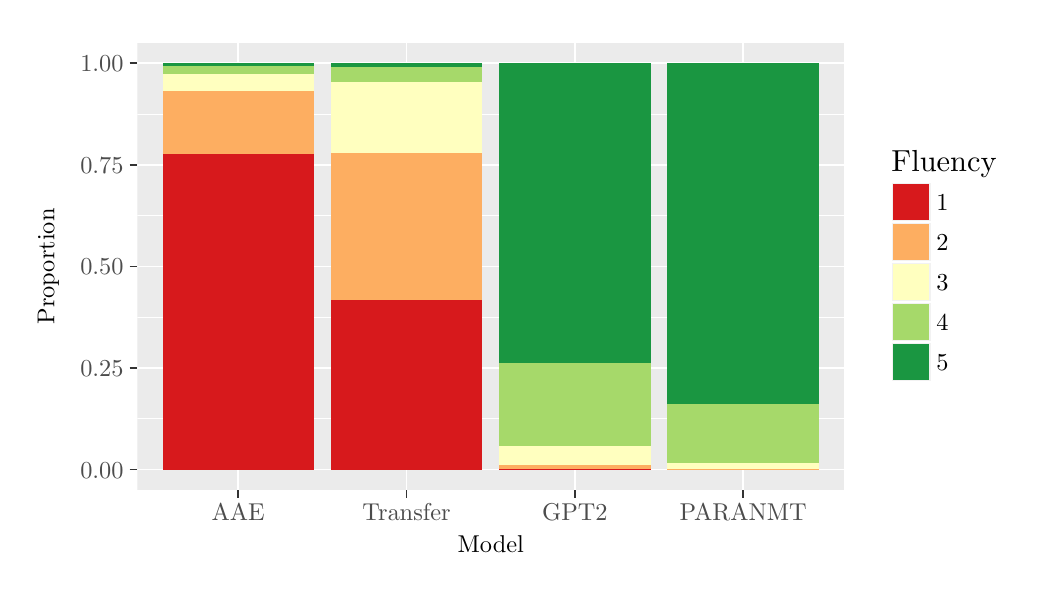
\begin{tikzpicture}[x=1pt,y=1pt]
\definecolor{fillColor}{RGB}{255,255,255}
\path[use as bounding box,fill=fillColor,fill opacity=0.00] (0,0) rectangle (361.35,195.13);
\begin{scope}
\path[clip] (  0.00,  0.00) rectangle (361.35,195.13);
\definecolor{drawColor}{RGB}{255,255,255}
\definecolor{fillColor}{RGB}{255,255,255}

\path[draw=drawColor,line width= 0.6pt,line join=round,line cap=round,fill=fillColor] (  0.00,  0.00) rectangle (361.35,195.13);
\end{scope}
\begin{scope}
\path[clip] ( 39.60, 28.07) rectangle (295.06,189.63);
\definecolor{fillColor}{gray}{0.92}

\path[fill=fillColor] ( 39.60, 28.07) rectangle (295.06,189.63);
\definecolor{drawColor}{RGB}{255,255,255}

\path[draw=drawColor,line width= 0.3pt,line join=round] ( 39.60, 53.77) --
	(295.06, 53.77);

\path[draw=drawColor,line width= 0.3pt,line join=round] ( 39.60, 90.49) --
	(295.06, 90.49);

\path[draw=drawColor,line width= 0.3pt,line join=round] ( 39.60,127.21) --
	(295.06,127.21);

\path[draw=drawColor,line width= 0.3pt,line join=round] ( 39.60,163.93) --
	(295.06,163.93);

\path[draw=drawColor,line width= 0.6pt,line join=round] ( 39.60, 35.42) --
	(295.06, 35.42);

\path[draw=drawColor,line width= 0.6pt,line join=round] ( 39.60, 72.13) --
	(295.06, 72.13);

\path[draw=drawColor,line width= 0.6pt,line join=round] ( 39.60,108.85) --
	(295.06,108.85);

\path[draw=drawColor,line width= 0.6pt,line join=round] ( 39.60,145.57) --
	(295.06,145.57);

\path[draw=drawColor,line width= 0.6pt,line join=round] ( 39.60,182.29) --
	(295.06,182.29);

\path[draw=drawColor,line width= 0.6pt,line join=round] ( 76.09, 28.07) --
	( 76.09,189.63);

\path[draw=drawColor,line width= 0.6pt,line join=round] (136.91, 28.07) --
	(136.91,189.63);

\path[draw=drawColor,line width= 0.6pt,line join=round] (197.74, 28.07) --
	(197.74,189.63);

\path[draw=drawColor,line width= 0.6pt,line join=round] (258.56, 28.07) --
	(258.56,189.63);
\definecolor{fillColor}{RGB}{215,25,28}

\path[fill=fillColor] ( 48.72, 35.42) rectangle (103.46,149.48);
\definecolor{fillColor}{RGB}{253,174,97}

\path[fill=fillColor] ( 48.72,149.48) rectangle (103.46,172.24);
\definecolor{fillColor}{RGB}{255,255,191}

\path[fill=fillColor] ( 48.72,172.24) rectangle (103.46,178.44);
\definecolor{fillColor}{RGB}{166,217,106}

\path[fill=fillColor] ( 48.72,178.44) rectangle (103.46,181.40);
\definecolor{fillColor}{RGB}{26,150,65}

\path[fill=fillColor] ( 48.72,181.40) rectangle (103.46,182.29);
\definecolor{fillColor}{RGB}{215,25,28}

\path[fill=fillColor] (109.54, 35.42) rectangle (164.28, 96.88);
\definecolor{fillColor}{RGB}{253,174,97}

\path[fill=fillColor] (109.54, 96.88) rectangle (164.28,149.78);
\definecolor{fillColor}{RGB}{255,255,191}

\path[fill=fillColor] (109.54,149.78) rectangle (164.28,175.49);
\definecolor{fillColor}{RGB}{166,217,106}

\path[fill=fillColor] (109.54,175.49) rectangle (164.28,180.81);
\definecolor{fillColor}{RGB}{26,150,65}

\path[fill=fillColor] (109.54,180.81) rectangle (164.28,182.29);
\definecolor{fillColor}{RGB}{215,25,28}

\path[fill=fillColor] (170.37, 35.42) rectangle (225.11, 35.71);
\definecolor{fillColor}{RGB}{253,174,97}

\path[fill=fillColor] (170.37, 35.71) rectangle (225.11, 37.19);
\definecolor{fillColor}{RGB}{255,255,191}

\path[fill=fillColor] (170.37, 37.19) rectangle (225.11, 43.98);
\definecolor{fillColor}{RGB}{166,217,106}

\path[fill=fillColor] (170.37, 43.98) rectangle (225.11, 73.83);
\definecolor{fillColor}{RGB}{26,150,65}

\path[fill=fillColor] (170.37, 73.83) rectangle (225.11,182.29);
\definecolor{fillColor}{RGB}{253,174,97}

\path[fill=fillColor] (231.19, 35.42) rectangle (285.93, 35.71);
\definecolor{fillColor}{RGB}{255,255,191}

\path[fill=fillColor] (231.19, 35.71) rectangle (285.93, 37.78);
\definecolor{fillColor}{RGB}{166,217,106}

\path[fill=fillColor] (231.19, 37.78) rectangle (285.93, 59.06);
\definecolor{fillColor}{RGB}{26,150,65}

\path[fill=fillColor] (231.19, 59.06) rectangle (285.93,182.29);
\end{scope}
\begin{scope}
\path[clip] (  0.00,  0.00) rectangle (361.35,195.13);
\definecolor{drawColor}{gray}{0.30}

\node[text=drawColor,anchor=base east,inner sep=0pt, outer sep=0pt, scale=  0.88] at ( 34.65, 32.38) {0.00};

\node[text=drawColor,anchor=base east,inner sep=0pt, outer sep=0pt, scale=  0.88] at ( 34.65, 69.10) {0.25};

\node[text=drawColor,anchor=base east,inner sep=0pt, outer sep=0pt, scale=  0.88] at ( 34.65,105.82) {0.50};

\node[text=drawColor,anchor=base east,inner sep=0pt, outer sep=0pt, scale=  0.88] at ( 34.65,142.54) {0.75};

\node[text=drawColor,anchor=base east,inner sep=0pt, outer sep=0pt, scale=  0.88] at ( 34.65,179.26) {1.00};
\end{scope}
\begin{scope}
\path[clip] (  0.00,  0.00) rectangle (361.35,195.13);
\definecolor{drawColor}{gray}{0.20}

\path[draw=drawColor,line width= 0.6pt,line join=round] ( 36.85, 35.42) --
	( 39.60, 35.42);

\path[draw=drawColor,line width= 0.6pt,line join=round] ( 36.85, 72.13) --
	( 39.60, 72.13);

\path[draw=drawColor,line width= 0.6pt,line join=round] ( 36.85,108.85) --
	( 39.60,108.85);

\path[draw=drawColor,line width= 0.6pt,line join=round] ( 36.85,145.57) --
	( 39.60,145.57);

\path[draw=drawColor,line width= 0.6pt,line join=round] ( 36.85,182.29) --
	( 39.60,182.29);
\end{scope}
\begin{scope}
\path[clip] (  0.00,  0.00) rectangle (361.35,195.13);
\definecolor{drawColor}{gray}{0.20}

\path[draw=drawColor,line width= 0.6pt,line join=round] ( 76.09, 25.32) --
	( 76.09, 28.07);

\path[draw=drawColor,line width= 0.6pt,line join=round] (136.91, 25.32) --
	(136.91, 28.07);

\path[draw=drawColor,line width= 0.6pt,line join=round] (197.74, 25.32) --
	(197.74, 28.07);

\path[draw=drawColor,line width= 0.6pt,line join=round] (258.56, 25.32) --
	(258.56, 28.07);
\end{scope}
\begin{scope}
\path[clip] (  0.00,  0.00) rectangle (361.35,195.13);
\definecolor{drawColor}{gray}{0.30}

\node[text=drawColor,anchor=base,inner sep=0pt, outer sep=0pt, scale=  0.88] at ( 76.09, 17.06) {AAE};

\node[text=drawColor,anchor=base,inner sep=0pt, outer sep=0pt, scale=  0.88] at (136.91, 17.06) {Transfer};

\node[text=drawColor,anchor=base,inner sep=0pt, outer sep=0pt, scale=  0.88] at (197.74, 17.06) {GPT2};

\node[text=drawColor,anchor=base,inner sep=0pt, outer sep=0pt, scale=  0.88] at (258.56, 17.06) {PARANMT};
\end{scope}
\begin{scope}
\path[clip] (  0.00,  0.00) rectangle (361.35,195.13);
\definecolor{drawColor}{RGB}{0,0,0}

\node[text=drawColor,anchor=base,inner sep=0pt, outer sep=0pt, scale=  0.88] at (167.33,  5.50) {Model};
\end{scope}
\begin{scope}
\path[clip] (  0.00,  0.00) rectangle (361.35,195.13);
\definecolor{drawColor}{RGB}{0,0,0}

\node[text=drawColor,rotate= 90.00,anchor=base,inner sep=0pt, outer sep=0pt, scale=  0.88] at (  9.62,108.85) {Proportion};
\end{scope}
\begin{scope}
\path[clip] (  0.00,  0.00) rectangle (361.35,195.13);
\definecolor{fillColor}{RGB}{255,255,255}

\path[fill=fillColor] (306.44, 61.43) rectangle (355.85,156.27);
\end{scope}
\begin{scope}
\path[clip] (  0.00,  0.00) rectangle (361.35,195.13);
\definecolor{drawColor}{RGB}{0,0,0}

\node[text=drawColor,anchor=base west,inner sep=0pt, outer sep=0pt, scale=  1.10] at (312.13,143.00) {Fluency};
\end{scope}
\begin{scope}
\path[clip] (  0.00,  0.00) rectangle (361.35,195.13);
\definecolor{drawColor}{RGB}{255,255,255}
\definecolor{fillColor}{gray}{0.95}

\path[draw=drawColor,line width= 0.6pt,line join=round,line cap=round,fill=fillColor] (312.13,124.94) rectangle (326.58,139.39);
\end{scope}
\begin{scope}
\path[clip] (  0.00,  0.00) rectangle (361.35,195.13);
\definecolor{fillColor}{RGB}{215,25,28}

\path[fill=fillColor] (312.84,125.65) rectangle (325.87,138.68);
\end{scope}
\begin{scope}
\path[clip] (  0.00,  0.00) rectangle (361.35,195.13);
\definecolor{drawColor}{RGB}{255,255,255}
\definecolor{fillColor}{gray}{0.95}

\path[draw=drawColor,line width= 0.6pt,line join=round,line cap=round,fill=fillColor] (312.13,110.48) rectangle (326.58,124.94);
\end{scope}
\begin{scope}
\path[clip] (  0.00,  0.00) rectangle (361.35,195.13);
\definecolor{fillColor}{RGB}{253,174,97}

\path[fill=fillColor] (312.84,111.19) rectangle (325.87,124.23);
\end{scope}
\begin{scope}
\path[clip] (  0.00,  0.00) rectangle (361.35,195.13);
\definecolor{drawColor}{RGB}{255,255,255}
\definecolor{fillColor}{gray}{0.95}

\path[draw=drawColor,line width= 0.6pt,line join=round,line cap=round,fill=fillColor] (312.13, 96.03) rectangle (326.58,110.48);
\end{scope}
\begin{scope}
\path[clip] (  0.00,  0.00) rectangle (361.35,195.13);
\definecolor{fillColor}{RGB}{255,255,191}

\path[fill=fillColor] (312.84, 96.74) rectangle (325.87,109.77);
\end{scope}
\begin{scope}
\path[clip] (  0.00,  0.00) rectangle (361.35,195.13);
\definecolor{drawColor}{RGB}{255,255,255}
\definecolor{fillColor}{gray}{0.95}

\path[draw=drawColor,line width= 0.6pt,line join=round,line cap=round,fill=fillColor] (312.13, 81.57) rectangle (326.58, 96.03);
\end{scope}
\begin{scope}
\path[clip] (  0.00,  0.00) rectangle (361.35,195.13);
\definecolor{fillColor}{RGB}{166,217,106}

\path[fill=fillColor] (312.84, 82.29) rectangle (325.87, 95.32);
\end{scope}
\begin{scope}
\path[clip] (  0.00,  0.00) rectangle (361.35,195.13);
\definecolor{drawColor}{RGB}{255,255,255}
\definecolor{fillColor}{gray}{0.95}

\path[draw=drawColor,line width= 0.6pt,line join=round,line cap=round,fill=fillColor] (312.13, 67.12) rectangle (326.58, 81.57);
\end{scope}
\begin{scope}
\path[clip] (  0.00,  0.00) rectangle (361.35,195.13);
\definecolor{fillColor}{RGB}{26,150,65}

\path[fill=fillColor] (312.84, 67.83) rectangle (325.87, 80.86);
\end{scope}
\begin{scope}
\path[clip] (  0.00,  0.00) rectangle (361.35,195.13);
\definecolor{drawColor}{RGB}{0,0,0}

\node[text=drawColor,anchor=base west,inner sep=0pt, outer sep=0pt, scale=  0.88] at (328.39,129.13) {1};
\end{scope}
\begin{scope}
\path[clip] (  0.00,  0.00) rectangle (361.35,195.13);
\definecolor{drawColor}{RGB}{0,0,0}

\node[text=drawColor,anchor=base west,inner sep=0pt, outer sep=0pt, scale=  0.88] at (328.39,114.68) {2};
\end{scope}
\begin{scope}
\path[clip] (  0.00,  0.00) rectangle (361.35,195.13);
\definecolor{drawColor}{RGB}{0,0,0}

\node[text=drawColor,anchor=base west,inner sep=0pt, outer sep=0pt, scale=  0.88] at (328.39,100.23) {3};
\end{scope}
\begin{scope}
\path[clip] (  0.00,  0.00) rectangle (361.35,195.13);
\definecolor{drawColor}{RGB}{0,0,0}

\node[text=drawColor,anchor=base west,inner sep=0pt, outer sep=0pt, scale=  0.88] at (328.39, 85.77) {4};
\end{scope}
\begin{scope}
\path[clip] (  0.00,  0.00) rectangle (361.35,195.13);
\definecolor{drawColor}{RGB}{0,0,0}

\node[text=drawColor,anchor=base west,inner sep=0pt, outer sep=0pt, scale=  0.88] at (328.39, 71.32) {5};
\end{scope}
\end{tikzpicture}

  \caption{Spread of user-evaluated fluency scores}
  \label{fluency}
\end{figure}



\begin{table}[h!]
\centering
  \vspace{4mm}
  \caption {User Study Results - Fluency} \label{fluencytable} 
  \vspace{2pt}
  \begin{tabular}{lrrrrrrr}
      \toprule
      \multirow{2}{*}{Source} &  \multirow{2}{*}{Mean Score} &  \multirow{2}{*}{$\sigma$} & \multicolumn{4}{c}{T Score}\\
      \cmidrule{4-7} 
      &&& AAE & Transfer & GPT2 & P{\footnotesize ARA}NMT\\
     \midrule
      AAE & 1.325 & 0.427      & - & 5.954** & 36.203** & 36.159** \\
      Transfer & 1.861 & 0.547      & - & -     & 27.072**  & 24.609** \\
      GPT2 & 4.668 & 0.225 & - & -     & -      & 4.212** \\
      Ground Truth & 4.820 & 0.219  & - & -     & -      & - \\
      \bottomrule
          \hline
  \end{tabular}
        \begin{flushright}
      \footnotesize{Note: $*p<.05$, **$p<.01$\hphantom{abcabaa}}
    \end{flushright}
    \vspace{-5mm}
\end{table}

% correlation between bleu and use scores

\section{Evaluation}

\noindent With regards to the aim of this paper, investigating the applications of cutting-edge NLP models to lexical steganography, we now discuss the strengths and limitations of each developed method, and their implications for the development of future systems.


\subsection{Adversarial Autoencoder}

\noindent By all measures, the adversarial autoencoder was not successful in its task, failing to encode even a single bit into the majority of tested samples. It may simply be the case that such a model is not suitable for this application, with Subramanian et al.\ (2018)\nocite{transfer} suggesting that the strong restrictions on the parametric form of the posterior may hamper the model's ability to encode information in the latent vector. While it may be possible to learn such a mapping for MNIST, attempting to do so for a distribution as discrete and high-dimensional as the English language is a problem so difficult that it takes priority over the reconstruction objective.

\begin{figure}[ht!]
  \centering
  \begin{subfigure}[t]{0.49\textwidth}
     \centering
      % Created by tikzDevice version 0.12 on 2019-04-30 13:33:07
% !TEX encoding = UTF-8 Unicode
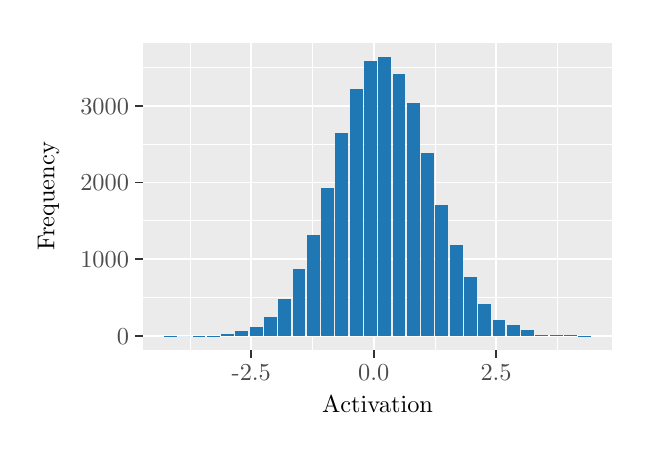
\begin{tikzpicture}[x=1pt,y=1pt]
\definecolor{fillColor}{RGB}{255,255,255}
\path[use as bounding box,fill=fillColor,fill opacity=0.00] (0,0) rectangle (216.81,144.54);
\begin{scope}
\path[clip] (  0.00,  0.00) rectangle (216.81,144.54);
\definecolor{drawColor}{RGB}{255,255,255}
\definecolor{fillColor}{RGB}{255,255,255}

\path[draw=drawColor,line width= 0.6pt,line join=round,line cap=round,fill=fillColor] (  0.00,  0.00) rectangle (216.81,144.54);
\end{scope}
\begin{scope}
\path[clip] ( 41.55, 28.07) rectangle (211.31,139.04);
\definecolor{fillColor}{gray}{0.92}

\path[fill=fillColor] ( 41.55, 28.07) rectangle (211.31,139.04);
\definecolor{drawColor}{RGB}{255,255,255}

\path[draw=drawColor,line width= 0.3pt,line join=round] ( 41.55, 46.98) --
	(211.31, 46.98);

\path[draw=drawColor,line width= 0.3pt,line join=round] ( 41.55, 74.72) --
	(211.31, 74.72);

\path[draw=drawColor,line width= 0.3pt,line join=round] ( 41.55,102.46) --
	(211.31,102.46);

\path[draw=drawColor,line width= 0.3pt,line join=round] ( 41.55,130.20) --
	(211.31,130.20);

\path[draw=drawColor,line width= 0.3pt,line join=round] ( 58.69, 28.07) --
	( 58.69,139.04);

\path[draw=drawColor,line width= 0.3pt,line join=round] (102.92, 28.07) --
	(102.92,139.04);

\path[draw=drawColor,line width= 0.3pt,line join=round] (147.16, 28.07) --
	(147.16,139.04);

\path[draw=drawColor,line width= 0.3pt,line join=round] (191.39, 28.07) --
	(191.39,139.04);

\path[draw=drawColor,line width= 0.6pt,line join=round] ( 41.55, 33.12) --
	(211.31, 33.12);

\path[draw=drawColor,line width= 0.6pt,line join=round] ( 41.55, 60.85) --
	(211.31, 60.85);

\path[draw=drawColor,line width= 0.6pt,line join=round] ( 41.55, 88.59) --
	(211.31, 88.59);

\path[draw=drawColor,line width= 0.6pt,line join=round] ( 41.55,116.33) --
	(211.31,116.33);

\path[draw=drawColor,line width= 0.6pt,line join=round] ( 80.81, 28.07) --
	( 80.81,139.04);

\path[draw=drawColor,line width= 0.6pt,line join=round] (125.04, 28.07) --
	(125.04,139.04);

\path[draw=drawColor,line width= 0.6pt,line join=round] (169.27, 28.07) --
	(169.27,139.04);
\definecolor{fillColor}{RGB}{31,120,180}

\path[fill=fillColor] ( 49.27, 33.12) rectangle ( 53.91, 33.14);

\path[fill=fillColor] ( 54.43, 33.12) rectangle ( 59.07, 33.12);

\path[fill=fillColor] ( 59.59, 33.12) rectangle ( 64.24, 33.17);

\path[fill=fillColor] ( 64.75, 33.12) rectangle ( 69.40, 33.23);

\path[fill=fillColor] ( 69.91, 33.12) rectangle ( 74.56, 33.67);

\path[fill=fillColor] ( 75.07, 33.12) rectangle ( 79.72, 34.95);

\path[fill=fillColor] ( 80.24, 33.12) rectangle ( 84.88, 36.47);

\path[fill=fillColor] ( 85.40, 33.12) rectangle ( 90.04, 39.94);

\path[fill=fillColor] ( 90.56, 33.12) rectangle ( 95.20, 46.65);

\path[fill=fillColor] ( 95.72, 33.12) rectangle (100.37, 57.44);

\path[fill=fillColor] (100.88, 33.12) rectangle (105.53, 69.56);

\path[fill=fillColor] (106.04, 33.12) rectangle (110.69, 86.65);

\path[fill=fillColor] (111.20, 33.12) rectangle (115.85,106.31);

\path[fill=fillColor] (116.37, 33.12) rectangle (121.01,122.40);

\path[fill=fillColor] (121.53, 33.12) rectangle (126.17,132.55);

\path[fill=fillColor] (126.69, 33.12) rectangle (131.33,134.00);

\path[fill=fillColor] (131.85, 33.12) rectangle (136.50,127.95);

\path[fill=fillColor] (137.01, 33.12) rectangle (141.66,117.49);

\path[fill=fillColor] (142.17, 33.12) rectangle (146.82, 99.27);

\path[fill=fillColor] (147.33, 33.12) rectangle (151.98, 80.44);

\path[fill=fillColor] (152.50, 33.12) rectangle (157.14, 65.93);

\path[fill=fillColor] (157.66, 33.12) rectangle (162.30, 54.56);

\path[fill=fillColor] (162.82, 33.12) rectangle (167.46, 44.79);

\path[fill=fillColor] (167.98, 33.12) rectangle (172.63, 39.00);

\path[fill=fillColor] (173.14, 33.12) rectangle (177.79, 36.94);

\path[fill=fillColor] (178.30, 33.12) rectangle (182.95, 35.36);

\path[fill=fillColor] (183.46, 33.12) rectangle (188.11, 33.64);

\path[fill=fillColor] (188.63, 33.12) rectangle (193.27, 33.48);

\path[fill=fillColor] (193.79, 33.12) rectangle (198.43, 33.31);

\path[fill=fillColor] (198.95, 33.12) rectangle (203.59, 33.23);
\end{scope}
\begin{scope}
\path[clip] (  0.00,  0.00) rectangle (216.81,144.54);
\definecolor{drawColor}{gray}{0.30}

\node[text=drawColor,anchor=base east,inner sep=0pt, outer sep=0pt, scale=  0.88] at ( 36.60, 30.09) {0};

\node[text=drawColor,anchor=base east,inner sep=0pt, outer sep=0pt, scale=  0.88] at ( 36.60, 57.82) {1000};

\node[text=drawColor,anchor=base east,inner sep=0pt, outer sep=0pt, scale=  0.88] at ( 36.60, 85.56) {2000};

\node[text=drawColor,anchor=base east,inner sep=0pt, outer sep=0pt, scale=  0.88] at ( 36.60,113.30) {3000};
\end{scope}
\begin{scope}
\path[clip] (  0.00,  0.00) rectangle (216.81,144.54);
\definecolor{drawColor}{gray}{0.20}

\path[draw=drawColor,line width= 0.6pt,line join=round] ( 38.80, 33.12) --
	( 41.55, 33.12);

\path[draw=drawColor,line width= 0.6pt,line join=round] ( 38.80, 60.85) --
	( 41.55, 60.85);

\path[draw=drawColor,line width= 0.6pt,line join=round] ( 38.80, 88.59) --
	( 41.55, 88.59);

\path[draw=drawColor,line width= 0.6pt,line join=round] ( 38.80,116.33) --
	( 41.55,116.33);
\end{scope}
\begin{scope}
\path[clip] (  0.00,  0.00) rectangle (216.81,144.54);
\definecolor{drawColor}{gray}{0.20}

\path[draw=drawColor,line width= 0.6pt,line join=round] ( 80.81, 25.32) --
	( 80.81, 28.07);

\path[draw=drawColor,line width= 0.6pt,line join=round] (125.04, 25.32) --
	(125.04, 28.07);

\path[draw=drawColor,line width= 0.6pt,line join=round] (169.27, 25.32) --
	(169.27, 28.07);
\end{scope}
\begin{scope}
\path[clip] (  0.00,  0.00) rectangle (216.81,144.54);
\definecolor{drawColor}{gray}{0.30}

\node[text=drawColor,anchor=base,inner sep=0pt, outer sep=0pt, scale=  0.88] at ( 80.81, 17.06) {-2.5};

\node[text=drawColor,anchor=base,inner sep=0pt, outer sep=0pt, scale=  0.88] at (125.04, 17.06) {0.0};

\node[text=drawColor,anchor=base,inner sep=0pt, outer sep=0pt, scale=  0.88] at (169.27, 17.06) {2.5};
\end{scope}
\begin{scope}
\path[clip] (  0.00,  0.00) rectangle (216.81,144.54);
\definecolor{drawColor}{RGB}{0,0,0}

\node[text=drawColor,anchor=base,inner sep=0pt, outer sep=0pt, scale=  0.88] at (126.43,  5.50) {Activation};
\end{scope}
\begin{scope}
\path[clip] (  0.00,  0.00) rectangle (216.81,144.54);
\definecolor{drawColor}{RGB}{0,0,0}

\node[text=drawColor,rotate= 90.00,anchor=base,inner sep=0pt, outer sep=0pt, scale=  0.88] at (  9.62, 83.56) {Frequency};
\end{scope}
\end{tikzpicture}

      \caption{}
      \label{good_hist}
  \end{subfigure}
  \hfill
  \begin{subfigure}[t]{0.49\textwidth}
         \centering
      % Created by tikzDevice version 0.12 on 2019-04-30 13:35:46
% !TEX encoding = UTF-8 Unicode
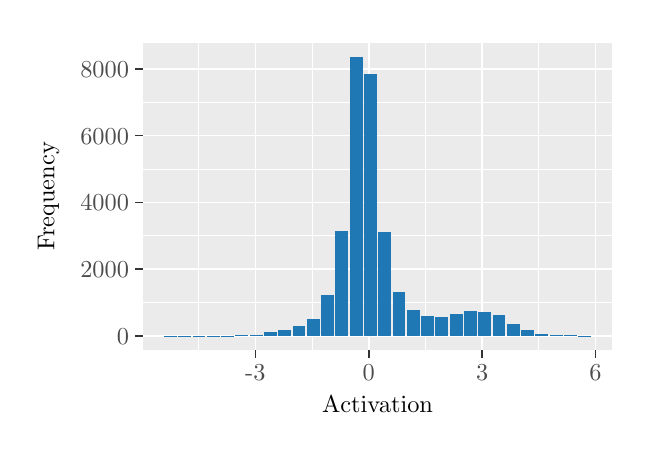
\begin{tikzpicture}[x=1pt,y=1pt]
\definecolor{fillColor}{RGB}{255,255,255}
\path[use as bounding box,fill=fillColor,fill opacity=0.00] (0,0) rectangle (216.81,144.54);
\begin{scope}
\path[clip] (  0.00,  0.00) rectangle (216.81,144.54);
\definecolor{drawColor}{RGB}{255,255,255}
\definecolor{fillColor}{RGB}{255,255,255}

\path[draw=drawColor,line width= 0.6pt,line join=round,line cap=round,fill=fillColor] (  0.00,  0.00) rectangle (216.81,144.54);
\end{scope}
\begin{scope}
\path[clip] ( 41.55, 28.07) rectangle (211.31,139.04);
\definecolor{fillColor}{gray}{0.92}

\path[fill=fillColor] ( 41.55, 28.07) rectangle (211.31,139.04);
\definecolor{drawColor}{RGB}{255,255,255}

\path[draw=drawColor,line width= 0.3pt,line join=round] ( 41.55, 45.18) --
	(211.31, 45.18);

\path[draw=drawColor,line width= 0.3pt,line join=round] ( 41.55, 69.32) --
	(211.31, 69.32);

\path[draw=drawColor,line width= 0.3pt,line join=round] ( 41.55, 93.46) --
	(211.31, 93.46);

\path[draw=drawColor,line width= 0.3pt,line join=round] ( 41.55,117.59) --
	(211.31,117.59);

\path[draw=drawColor,line width= 0.3pt,line join=round] ( 61.79, 28.07) --
	( 61.79,139.04);

\path[draw=drawColor,line width= 0.3pt,line join=round] (102.76, 28.07) --
	(102.76,139.04);

\path[draw=drawColor,line width= 0.3pt,line join=round] (143.73, 28.07) --
	(143.73,139.04);

\path[draw=drawColor,line width= 0.3pt,line join=round] (184.70, 28.07) --
	(184.70,139.04);

\path[draw=drawColor,line width= 0.6pt,line join=round] ( 41.55, 33.12) --
	(211.31, 33.12);

\path[draw=drawColor,line width= 0.6pt,line join=round] ( 41.55, 57.25) --
	(211.31, 57.25);

\path[draw=drawColor,line width= 0.6pt,line join=round] ( 41.55, 81.39) --
	(211.31, 81.39);

\path[draw=drawColor,line width= 0.6pt,line join=round] ( 41.55,105.53) --
	(211.31,105.53);

\path[draw=drawColor,line width= 0.6pt,line join=round] ( 41.55,129.66) --
	(211.31,129.66);

\path[draw=drawColor,line width= 0.6pt,line join=round] ( 82.28, 28.07) --
	( 82.28,139.04);

\path[draw=drawColor,line width= 0.6pt,line join=round] (123.25, 28.07) --
	(123.25,139.04);

\path[draw=drawColor,line width= 0.6pt,line join=round] (164.22, 28.07) --
	(164.22,139.04);

\path[draw=drawColor,line width= 0.6pt,line join=round] (205.19, 28.07) --
	(205.19,139.04);
\definecolor{fillColor}{RGB}{31,120,180}

\path[fill=fillColor] ( 49.27, 33.12) rectangle ( 53.91, 33.13);

\path[fill=fillColor] ( 54.43, 33.12) rectangle ( 59.07, 33.14);

\path[fill=fillColor] ( 59.59, 33.12) rectangle ( 64.24, 33.15);

\path[fill=fillColor] ( 64.75, 33.12) rectangle ( 69.40, 33.19);

\path[fill=fillColor] ( 69.91, 33.12) rectangle ( 74.56, 33.25);

\path[fill=fillColor] ( 75.07, 33.12) rectangle ( 79.72, 33.43);

\path[fill=fillColor] ( 80.24, 33.12) rectangle ( 84.88, 33.63);

\path[fill=fillColor] ( 85.40, 33.12) rectangle ( 90.04, 34.46);

\path[fill=fillColor] ( 90.56, 33.12) rectangle ( 95.20, 35.19);

\path[fill=fillColor] ( 95.72, 33.12) rectangle (100.37, 36.63);

\path[fill=fillColor] (100.88, 33.12) rectangle (105.53, 39.22);

\path[fill=fillColor] (106.04, 33.12) rectangle (110.69, 48.02);

\path[fill=fillColor] (111.20, 33.12) rectangle (115.85, 71.00);

\path[fill=fillColor] (116.37, 33.12) rectangle (121.01,134.00);

\path[fill=fillColor] (121.53, 33.12) rectangle (126.17,127.62);

\path[fill=fillColor] (126.69, 33.12) rectangle (131.33, 70.77);

\path[fill=fillColor] (131.85, 33.12) rectangle (136.50, 49.07);

\path[fill=fillColor] (137.01, 33.12) rectangle (141.66, 42.44);

\path[fill=fillColor] (142.17, 33.12) rectangle (146.82, 40.38);

\path[fill=fillColor] (147.33, 33.12) rectangle (151.98, 40.12);

\path[fill=fillColor] (152.50, 33.12) rectangle (157.14, 41.04);

\path[fill=fillColor] (157.66, 33.12) rectangle (162.30, 42.11);

\path[fill=fillColor] (162.82, 33.12) rectangle (167.46, 41.88);

\path[fill=fillColor] (167.98, 33.12) rectangle (172.63, 40.60);

\path[fill=fillColor] (173.14, 33.12) rectangle (177.79, 37.58);

\path[fill=fillColor] (178.30, 33.12) rectangle (182.95, 35.24);

\path[fill=fillColor] (183.46, 33.12) rectangle (188.11, 33.95);

\path[fill=fillColor] (188.63, 33.12) rectangle (193.27, 33.55);

\path[fill=fillColor] (193.79, 33.12) rectangle (198.43, 33.33);

\path[fill=fillColor] (198.95, 33.12) rectangle (203.59, 33.14);
\end{scope}
\begin{scope}
\path[clip] (  0.00,  0.00) rectangle (216.81,144.54);
\definecolor{drawColor}{gray}{0.30}

\node[text=drawColor,anchor=base east,inner sep=0pt, outer sep=0pt, scale=  0.88] at ( 36.60, 30.09) {0};

\node[text=drawColor,anchor=base east,inner sep=0pt, outer sep=0pt, scale=  0.88] at ( 36.60, 54.22) {2000};

\node[text=drawColor,anchor=base east,inner sep=0pt, outer sep=0pt, scale=  0.88] at ( 36.60, 78.36) {4000};

\node[text=drawColor,anchor=base east,inner sep=0pt, outer sep=0pt, scale=  0.88] at ( 36.60,102.50) {6000};

\node[text=drawColor,anchor=base east,inner sep=0pt, outer sep=0pt, scale=  0.88] at ( 36.60,126.63) {8000};
\end{scope}
\begin{scope}
\path[clip] (  0.00,  0.00) rectangle (216.81,144.54);
\definecolor{drawColor}{gray}{0.20}

\path[draw=drawColor,line width= 0.6pt,line join=round] ( 38.80, 33.12) --
	( 41.55, 33.12);

\path[draw=drawColor,line width= 0.6pt,line join=round] ( 38.80, 57.25) --
	( 41.55, 57.25);

\path[draw=drawColor,line width= 0.6pt,line join=round] ( 38.80, 81.39) --
	( 41.55, 81.39);

\path[draw=drawColor,line width= 0.6pt,line join=round] ( 38.80,105.53) --
	( 41.55,105.53);

\path[draw=drawColor,line width= 0.6pt,line join=round] ( 38.80,129.66) --
	( 41.55,129.66);
\end{scope}
\begin{scope}
\path[clip] (  0.00,  0.00) rectangle (216.81,144.54);
\definecolor{drawColor}{gray}{0.20}

\path[draw=drawColor,line width= 0.6pt,line join=round] ( 82.28, 25.32) --
	( 82.28, 28.07);

\path[draw=drawColor,line width= 0.6pt,line join=round] (123.25, 25.32) --
	(123.25, 28.07);

\path[draw=drawColor,line width= 0.6pt,line join=round] (164.22, 25.32) --
	(164.22, 28.07);

\path[draw=drawColor,line width= 0.6pt,line join=round] (205.19, 25.32) --
	(205.19, 28.07);
\end{scope}
\begin{scope}
\path[clip] (  0.00,  0.00) rectangle (216.81,144.54);
\definecolor{drawColor}{gray}{0.30}

\node[text=drawColor,anchor=base,inner sep=0pt, outer sep=0pt, scale=  0.88] at ( 82.28, 17.06) {-3};

\node[text=drawColor,anchor=base,inner sep=0pt, outer sep=0pt, scale=  0.88] at (123.25, 17.06) {0};

\node[text=drawColor,anchor=base,inner sep=0pt, outer sep=0pt, scale=  0.88] at (164.22, 17.06) {3};

\node[text=drawColor,anchor=base,inner sep=0pt, outer sep=0pt, scale=  0.88] at (205.19, 17.06) {6};
\end{scope}
\begin{scope}
\path[clip] (  0.00,  0.00) rectangle (216.81,144.54);
\definecolor{drawColor}{RGB}{0,0,0}

\node[text=drawColor,anchor=base,inner sep=0pt, outer sep=0pt, scale=  0.88] at (126.43,  5.50) {Activation};
\end{scope}
\begin{scope}
\path[clip] (  0.00,  0.00) rectangle (216.81,144.54);
\definecolor{drawColor}{RGB}{0,0,0}

\node[text=drawColor,rotate= 90.00,anchor=base,inner sep=0pt, outer sep=0pt, scale=  0.88] at (  9.62, 83.56) {Frequency};
\end{scope}
\end{tikzpicture}

      \caption{}
      \label{bad_hist}
  \end{subfigure}
  \caption{Aggregate posteriors for the AAE model trained at $\alpha$ = 1 (a) and 0.0001 (b) }
  \label{hists}
\end{figure}

\begin{figure}[htp!]
  \centering
  \begin{subfigure}[t]{0.49\textwidth}
         \centering
      % Created by tikzDevice version 0.12 on 2019-04-30 14:04:11
% !TEX encoding = UTF-8 Unicode
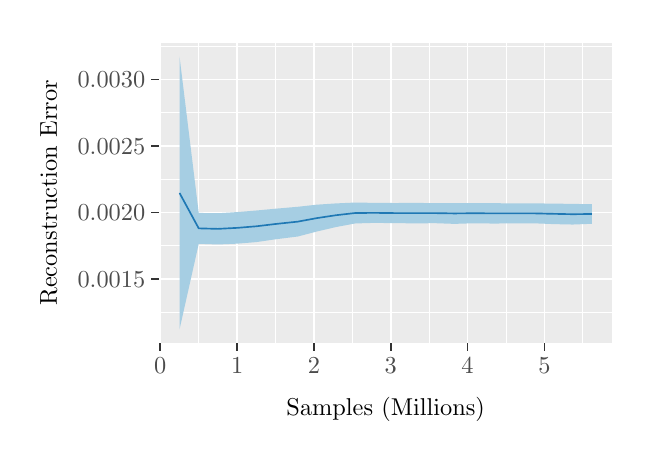
\begin{tikzpicture}[x=1pt,y=1pt]
\definecolor{fillColor}{RGB}{255,255,255}
\path[use as bounding box,fill=fillColor,fill opacity=0.00] (0,0) rectangle (216.81,144.54);
\begin{scope}
\path[clip] (  0.00,  0.00) rectangle (216.81,144.54);
\definecolor{drawColor}{RGB}{255,255,255}
\definecolor{fillColor}{RGB}{255,255,255}

\path[draw=drawColor,line width= 0.6pt,line join=round,line cap=round,fill=fillColor] (  0.00,  0.00) rectangle (216.81,144.54);
\end{scope}
\begin{scope}
\path[clip] ( 47.42, 30.57) rectangle (211.31,139.04);
\definecolor{fillColor}{gray}{0.92}

\path[fill=fillColor] ( 47.42, 30.57) rectangle (211.31,139.04);
\definecolor{drawColor}{RGB}{255,255,255}

\path[draw=drawColor,line width= 0.3pt,line join=round] ( 47.42, 41.80) --
	(211.31, 41.80);

\path[draw=drawColor,line width= 0.3pt,line join=round] ( 47.42, 65.79) --
	(211.31, 65.79);

\path[draw=drawColor,line width= 0.3pt,line join=round] ( 47.42, 89.79) --
	(211.31, 89.79);

\path[draw=drawColor,line width= 0.3pt,line join=round] ( 47.42,113.78) --
	(211.31,113.78);

\path[draw=drawColor,line width= 0.3pt,line join=round] ( 47.42,137.78) --
	(211.31,137.78);

\path[draw=drawColor,line width= 0.3pt,line join=round] ( 61.81, 30.57) --
	( 61.81,139.04);

\path[draw=drawColor,line width= 0.3pt,line join=round] ( 89.57, 30.57) --
	( 89.57,139.04);

\path[draw=drawColor,line width= 0.3pt,line join=round] (117.32, 30.57) --
	(117.32,139.04);

\path[draw=drawColor,line width= 0.3pt,line join=round] (145.08, 30.57) --
	(145.08,139.04);

\path[draw=drawColor,line width= 0.3pt,line join=round] (172.84, 30.57) --
	(172.84,139.04);

\path[draw=drawColor,line width= 0.3pt,line join=round] (200.60, 30.57) --
	(200.60,139.04);

\path[draw=drawColor,line width= 0.6pt,line join=round] ( 47.42, 53.79) --
	(211.31, 53.79);

\path[draw=drawColor,line width= 0.6pt,line join=round] ( 47.42, 77.79) --
	(211.31, 77.79);

\path[draw=drawColor,line width= 0.6pt,line join=round] ( 47.42,101.78) --
	(211.31,101.78);

\path[draw=drawColor,line width= 0.6pt,line join=round] ( 47.42,125.78) --
	(211.31,125.78);

\path[draw=drawColor,line width= 0.6pt,line join=round] ( 47.93, 30.57) --
	( 47.93,139.04);

\path[draw=drawColor,line width= 0.6pt,line join=round] ( 75.69, 30.57) --
	( 75.69,139.04);

\path[draw=drawColor,line width= 0.6pt,line join=round] (103.45, 30.57) --
	(103.45,139.04);

\path[draw=drawColor,line width= 0.6pt,line join=round] (131.20, 30.57) --
	(131.20,139.04);

\path[draw=drawColor,line width= 0.6pt,line join=round] (158.96, 30.57) --
	(158.96,139.04);

\path[draw=drawColor,line width= 0.6pt,line join=round] (186.72, 30.57) --
	(186.72,139.04);
\definecolor{fillColor}{RGB}{166,206,227}

\path[fill=fillColor] ( 54.87,134.11) --
	( 61.81, 77.60) --
	( 68.75, 77.48) --
	( 75.69, 77.90) --
	( 82.63, 78.47) --
	( 89.57, 79.12) --
	( 97.60, 79.82) --
	(104.53, 80.58) --
	(111.47, 81.04) --
	(118.41, 81.35) --
	(125.35, 81.23) --
	(132.29, 81.18) --
	(140.32, 81.20) --
	(147.26, 81.16) --
	(154.20, 81.17) --
	(161.14, 81.10) --
	(168.08, 81.11) --
	(175.01, 81.07) --
	(183.04, 81.03) --
	(189.98, 80.98) --
	(196.92, 80.85) --
	(203.86, 80.77) --
	(203.86, 73.67) --
	(196.92, 73.40) --
	(189.98, 73.56) --
	(183.04, 73.84) --
	(175.01, 73.81) --
	(168.08, 73.76) --
	(161.14, 73.86) --
	(154.20, 73.64) --
	(147.26, 73.89) --
	(140.32, 73.83) --
	(132.29, 73.91) --
	(125.35, 74.00) --
	(118.41, 73.80) --
	(111.47, 72.51) --
	(104.53, 70.89) --
	( 97.60, 69.07) --
	( 89.57, 68.07) --
	( 82.63, 67.06) --
	( 75.69, 66.49) --
	( 68.75, 66.20) --
	( 61.81, 66.45) --
	( 54.87, 35.50) --
	cycle;
\definecolor{drawColor}{RGB}{31,120,180}

\path[draw=drawColor,line width= 0.6pt,line join=round] ( 54.87, 84.81) --
	( 61.81, 72.02) --
	( 68.75, 71.84) --
	( 75.69, 72.20) --
	( 82.63, 72.77) --
	( 89.57, 73.60) --
	( 97.60, 74.45) --
	(104.53, 75.73) --
	(111.47, 76.78) --
	(118.41, 77.57) --
	(125.35, 77.62) --
	(132.29, 77.54) --
	(140.32, 77.51) --
	(147.26, 77.52) --
	(154.20, 77.41) --
	(161.14, 77.48) --
	(168.08, 77.43) --
	(175.01, 77.44) --
	(183.04, 77.43) --
	(189.98, 77.27) --
	(196.92, 77.13) --
	(203.86, 77.22);
\end{scope}
\begin{scope}
\path[clip] (  0.00,  0.00) rectangle (216.81,144.54);
\definecolor{drawColor}{gray}{0.30}

\node[text=drawColor,anchor=base east,inner sep=0pt, outer sep=0pt, scale=  0.88] at ( 42.47, 50.76) {0.0015};

\node[text=drawColor,anchor=base east,inner sep=0pt, outer sep=0pt, scale=  0.88] at ( 42.47, 74.76) {0.0020};

\node[text=drawColor,anchor=base east,inner sep=0pt, outer sep=0pt, scale=  0.88] at ( 42.47, 98.75) {0.0025};

\node[text=drawColor,anchor=base east,inner sep=0pt, outer sep=0pt, scale=  0.88] at ( 42.47,122.75) {0.0030};
\end{scope}
\begin{scope}
\path[clip] (  0.00,  0.00) rectangle (216.81,144.54);
\definecolor{drawColor}{gray}{0.20}

\path[draw=drawColor,line width= 0.6pt,line join=round] ( 44.67, 53.79) --
	( 47.42, 53.79);

\path[draw=drawColor,line width= 0.6pt,line join=round] ( 44.67, 77.79) --
	( 47.42, 77.79);

\path[draw=drawColor,line width= 0.6pt,line join=round] ( 44.67,101.78) --
	( 47.42,101.78);

\path[draw=drawColor,line width= 0.6pt,line join=round] ( 44.67,125.78) --
	( 47.42,125.78);
\end{scope}
\begin{scope}
\path[clip] (  0.00,  0.00) rectangle (216.81,144.54);
\definecolor{drawColor}{gray}{0.20}

\path[draw=drawColor,line width= 0.6pt,line join=round] ( 47.93, 27.82) --
	( 47.93, 30.57);

\path[draw=drawColor,line width= 0.6pt,line join=round] ( 75.69, 27.82) --
	( 75.69, 30.57);

\path[draw=drawColor,line width= 0.6pt,line join=round] (103.45, 27.82) --
	(103.45, 30.57);

\path[draw=drawColor,line width= 0.6pt,line join=round] (131.20, 27.82) --
	(131.20, 30.57);

\path[draw=drawColor,line width= 0.6pt,line join=round] (158.96, 27.82) --
	(158.96, 30.57);

\path[draw=drawColor,line width= 0.6pt,line join=round] (186.72, 27.82) --
	(186.72, 30.57);
\end{scope}
\begin{scope}
\path[clip] (  0.00,  0.00) rectangle (216.81,144.54);
\definecolor{drawColor}{gray}{0.30}

\node[text=drawColor,anchor=base,inner sep=0pt, outer sep=0pt, scale=  0.88] at ( 47.93, 19.56) {0};

\node[text=drawColor,anchor=base,inner sep=0pt, outer sep=0pt, scale=  0.88] at ( 75.69, 19.56) {1};

\node[text=drawColor,anchor=base,inner sep=0pt, outer sep=0pt, scale=  0.88] at (103.45, 19.56) {2};

\node[text=drawColor,anchor=base,inner sep=0pt, outer sep=0pt, scale=  0.88] at (131.20, 19.56) {3};

\node[text=drawColor,anchor=base,inner sep=0pt, outer sep=0pt, scale=  0.88] at (158.96, 19.56) {4};

\node[text=drawColor,anchor=base,inner sep=0pt, outer sep=0pt, scale=  0.88] at (186.72, 19.56) {5};
\end{scope}
\begin{scope}
\path[clip] (  0.00,  0.00) rectangle (216.81,144.54);
\definecolor{drawColor}{RGB}{0,0,0}

\node[text=drawColor,anchor=base,inner sep=0pt, outer sep=0pt, scale=  0.88] at (129.37,  4.25) {Samples (Millions)};
\end{scope}
\begin{scope}
\path[clip] (  0.00,  0.00) rectangle (216.81,144.54);
\definecolor{drawColor}{RGB}{0,0,0}

\node[text=drawColor,rotate= 90.00,anchor=base,inner sep=0pt, outer sep=0pt, scale=  0.88] at ( 10.59, 84.81) {Reconstruction Error};
\end{scope}
\end{tikzpicture}

      \caption{}
      \label{good_line}
  \end{subfigure}
  \hfill
  \begin{subfigure}[t]{0.49\textwidth}
         \centering
      % Created by tikzDevice version 0.12 on 2019-04-30 14:04:59
% !TEX encoding = UTF-8 Unicode
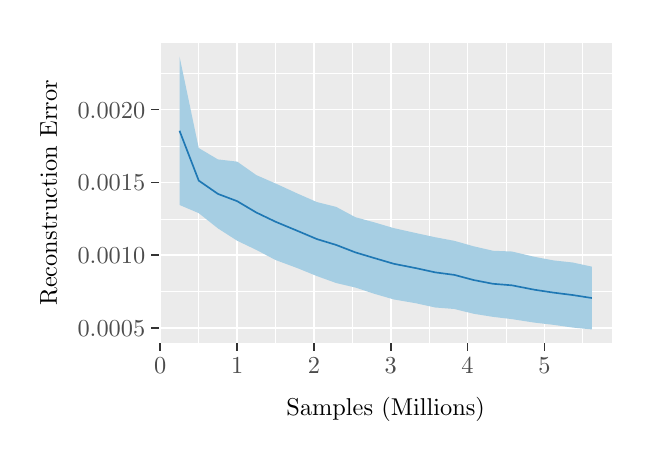
\begin{tikzpicture}[x=1pt,y=1pt]
\definecolor{fillColor}{RGB}{255,255,255}
\path[use as bounding box,fill=fillColor,fill opacity=0.00] (0,0) rectangle (216.81,144.54);
\begin{scope}
\path[clip] (  0.00,  0.00) rectangle (216.81,144.54);
\definecolor{drawColor}{RGB}{255,255,255}
\definecolor{fillColor}{RGB}{255,255,255}

\path[draw=drawColor,line width= 0.6pt,line join=round,line cap=round,fill=fillColor] (  0.00,  0.00) rectangle (216.81,144.54);
\end{scope}
\begin{scope}
\path[clip] ( 47.42, 30.57) rectangle (211.31,139.04);
\definecolor{fillColor}{gray}{0.92}

\path[fill=fillColor] ( 47.42, 30.57) rectangle (211.31,139.04);
\definecolor{drawColor}{RGB}{255,255,255}

\path[draw=drawColor,line width= 0.3pt,line join=round] ( 47.42, 49.12) --
	(211.31, 49.12);

\path[draw=drawColor,line width= 0.3pt,line join=round] ( 47.42, 75.43) --
	(211.31, 75.43);

\path[draw=drawColor,line width= 0.3pt,line join=round] ( 47.42,101.75) --
	(211.31,101.75);

\path[draw=drawColor,line width= 0.3pt,line join=round] ( 47.42,128.07) --
	(211.31,128.07);

\path[draw=drawColor,line width= 0.3pt,line join=round] ( 61.81, 30.57) --
	( 61.81,139.04);

\path[draw=drawColor,line width= 0.3pt,line join=round] ( 89.57, 30.57) --
	( 89.57,139.04);

\path[draw=drawColor,line width= 0.3pt,line join=round] (117.32, 30.57) --
	(117.32,139.04);

\path[draw=drawColor,line width= 0.3pt,line join=round] (145.08, 30.57) --
	(145.08,139.04);

\path[draw=drawColor,line width= 0.3pt,line join=round] (172.84, 30.57) --
	(172.84,139.04);

\path[draw=drawColor,line width= 0.3pt,line join=round] (200.60, 30.57) --
	(200.60,139.04);

\path[draw=drawColor,line width= 0.6pt,line join=round] ( 47.42, 35.96) --
	(211.31, 35.96);

\path[draw=drawColor,line width= 0.6pt,line join=round] ( 47.42, 62.28) --
	(211.31, 62.28);

\path[draw=drawColor,line width= 0.6pt,line join=round] ( 47.42, 88.59) --
	(211.31, 88.59);

\path[draw=drawColor,line width= 0.6pt,line join=round] ( 47.42,114.91) --
	(211.31,114.91);

\path[draw=drawColor,line width= 0.6pt,line join=round] ( 47.93, 30.57) --
	( 47.93,139.04);

\path[draw=drawColor,line width= 0.6pt,line join=round] ( 75.69, 30.57) --
	( 75.69,139.04);

\path[draw=drawColor,line width= 0.6pt,line join=round] (103.45, 30.57) --
	(103.45,139.04);

\path[draw=drawColor,line width= 0.6pt,line join=round] (131.20, 30.57) --
	(131.20,139.04);

\path[draw=drawColor,line width= 0.6pt,line join=round] (158.96, 30.57) --
	(158.96,139.04);

\path[draw=drawColor,line width= 0.6pt,line join=round] (186.72, 30.57) --
	(186.72,139.04);
\definecolor{fillColor}{RGB}{166,206,227}

\path[fill=fillColor] ( 54.87,134.11) --
	( 61.81,101.05) --
	( 68.75, 96.93) --
	( 75.69, 96.14) --
	( 82.63, 91.26) --
	( 89.57, 88.24) --
	( 97.60, 84.55) --
	(104.53, 81.51) --
	(111.47, 79.78) --
	(118.41, 76.05) --
	(125.35, 74.16) --
	(132.29, 72.10) --
	(140.32, 70.32) --
	(147.26, 68.81) --
	(154.20, 67.51) --
	(161.14, 65.54) --
	(168.08, 63.94) --
	(175.01, 63.65) --
	(183.04, 61.75) --
	(189.98, 60.44) --
	(196.92, 59.69) --
	(203.86, 58.19) --
	(203.86, 35.50) --
	(196.92, 36.18) --
	(189.98, 37.16) --
	(183.04, 37.97) --
	(175.01, 39.22) --
	(168.08, 40.05) --
	(161.14, 41.16) --
	(154.20, 42.88) --
	(147.26, 43.43) --
	(140.32, 44.95) --
	(132.29, 46.34) --
	(125.35, 48.35) --
	(118.41, 50.64) --
	(111.47, 52.27) --
	(104.53, 54.77) --
	( 97.60, 57.60) --
	( 89.57, 60.58) --
	( 82.63, 64.23) --
	( 75.69, 67.56) --
	( 68.75, 72.01) --
	( 61.81, 77.52) --
	( 54.87, 80.47) --
	cycle;
\definecolor{drawColor}{RGB}{31,120,180}

\path[draw=drawColor,line width= 0.6pt,line join=round] ( 54.87,107.29) --
	( 61.81, 89.28) --
	( 68.75, 84.47) --
	( 75.69, 81.85) --
	( 82.63, 77.74) --
	( 89.57, 74.41) --
	( 97.60, 71.07) --
	(104.53, 68.14) --
	(111.47, 66.03) --
	(118.41, 63.34) --
	(125.35, 61.26) --
	(132.29, 59.22) --
	(140.32, 57.64) --
	(147.26, 56.12) --
	(154.20, 55.20) --
	(161.14, 53.35) --
	(168.08, 52.00) --
	(175.01, 51.43) --
	(183.04, 49.86) --
	(189.98, 48.80) --
	(196.92, 47.93) --
	(203.86, 46.85);
\end{scope}
\begin{scope}
\path[clip] (  0.00,  0.00) rectangle (216.81,144.54);
\definecolor{drawColor}{gray}{0.30}

\node[text=drawColor,anchor=base east,inner sep=0pt, outer sep=0pt, scale=  0.88] at ( 42.47, 32.93) {0.0005};

\node[text=drawColor,anchor=base east,inner sep=0pt, outer sep=0pt, scale=  0.88] at ( 42.47, 59.24) {0.0010};

\node[text=drawColor,anchor=base east,inner sep=0pt, outer sep=0pt, scale=  0.88] at ( 42.47, 85.56) {0.0015};

\node[text=drawColor,anchor=base east,inner sep=0pt, outer sep=0pt, scale=  0.88] at ( 42.47,111.88) {0.0020};
\end{scope}
\begin{scope}
\path[clip] (  0.00,  0.00) rectangle (216.81,144.54);
\definecolor{drawColor}{gray}{0.20}

\path[draw=drawColor,line width= 0.6pt,line join=round] ( 44.67, 35.96) --
	( 47.42, 35.96);

\path[draw=drawColor,line width= 0.6pt,line join=round] ( 44.67, 62.28) --
	( 47.42, 62.28);

\path[draw=drawColor,line width= 0.6pt,line join=round] ( 44.67, 88.59) --
	( 47.42, 88.59);

\path[draw=drawColor,line width= 0.6pt,line join=round] ( 44.67,114.91) --
	( 47.42,114.91);
\end{scope}
\begin{scope}
\path[clip] (  0.00,  0.00) rectangle (216.81,144.54);
\definecolor{drawColor}{gray}{0.20}

\path[draw=drawColor,line width= 0.6pt,line join=round] ( 47.93, 27.82) --
	( 47.93, 30.57);

\path[draw=drawColor,line width= 0.6pt,line join=round] ( 75.69, 27.82) --
	( 75.69, 30.57);

\path[draw=drawColor,line width= 0.6pt,line join=round] (103.45, 27.82) --
	(103.45, 30.57);

\path[draw=drawColor,line width= 0.6pt,line join=round] (131.20, 27.82) --
	(131.20, 30.57);

\path[draw=drawColor,line width= 0.6pt,line join=round] (158.96, 27.82) --
	(158.96, 30.57);

\path[draw=drawColor,line width= 0.6pt,line join=round] (186.72, 27.82) --
	(186.72, 30.57);
\end{scope}
\begin{scope}
\path[clip] (  0.00,  0.00) rectangle (216.81,144.54);
\definecolor{drawColor}{gray}{0.30}

\node[text=drawColor,anchor=base,inner sep=0pt, outer sep=0pt, scale=  0.88] at ( 47.93, 19.56) {0};

\node[text=drawColor,anchor=base,inner sep=0pt, outer sep=0pt, scale=  0.88] at ( 75.69, 19.56) {1};

\node[text=drawColor,anchor=base,inner sep=0pt, outer sep=0pt, scale=  0.88] at (103.45, 19.56) {2};

\node[text=drawColor,anchor=base,inner sep=0pt, outer sep=0pt, scale=  0.88] at (131.20, 19.56) {3};

\node[text=drawColor,anchor=base,inner sep=0pt, outer sep=0pt, scale=  0.88] at (158.96, 19.56) {4};

\node[text=drawColor,anchor=base,inner sep=0pt, outer sep=0pt, scale=  0.88] at (186.72, 19.56) {5};
\end{scope}
\begin{scope}
\path[clip] (  0.00,  0.00) rectangle (216.81,144.54);
\definecolor{drawColor}{RGB}{0,0,0}

\node[text=drawColor,anchor=base,inner sep=0pt, outer sep=0pt, scale=  0.88] at (129.37,  4.25) {Samples (Millions)};
\end{scope}
\begin{scope}
\path[clip] (  0.00,  0.00) rectangle (216.81,144.54);
\definecolor{drawColor}{RGB}{0,0,0}

\node[text=drawColor,rotate= 90.00,anchor=base,inner sep=0pt, outer sep=0pt, scale=  0.88] at ( 10.59, 84.81) {Reconstruction Error};
\end{scope}
\end{tikzpicture}

      \caption{}
      \label{bad_line}
  \end{subfigure}
  \caption{Reconstruction error (training) for the AAE model trained at $\alpha$ = 1 (a) and 0.0001 (b)}
  \label{lines}
\end{figure}

This problem quickly became evident during training as the model appeared to be highly sensitive to changes in $\alpha$, the weight of the posterior regularisation term . As shown in Figures \ref{hists} and \ref{lines}, when the loss terms were equally weighted, the model experienced `posterior collapse' \cite{cont}, forcing the latent encoding to follow the correct distribution at the expense of ignoring the reconstruction term completely. Lowering the weight resulted in a sharp transition to the opposite problem, with there appearing to be no point at which the model would optimise both objectives in tandem. The behaviour of the model in its current form additionally suggests that the reconstruction objective does not lend itself well to paraphrase generation. Sampling around a particular point would often result in the same `base sentence' varied around its most uncommon word, usually changing the meaning of the sentence significantly.

% While it is likely that because of these issues, an adversarial autoencoder cannot be applied to the problem of lexical steganography, it must be noted that the effectiveness of the model was limited by technological constraints. Since the model was trained

% - mse loss function
%   - reconstruction objective does not work as a proxy
% - posterior collapse
% - small dataset 1.5M tweets

\subsection{Transfer Learning Autoencoder}

\noindent While the transfer learning model did appear to generalise more easily to unseen data than the adversarial autoencoder, the gradient-based interpolation schemes struggled to generate a large number of fluent paraphrases. This suggests that paraphrases do not necessarily occupy the same local area, and thus the gradient-based approaches are unlikely to find them. This idea is further supported by the relative success of the analogical interpretation scheme, which does not limit itself to any particular area of the latent space. The analogical method does however make the assumption that the latent space has a set of globally consistent `paraphrase vectors'. The partial success of the analogical method suggests that this assumption is true to a certain extent, but it is more likely that the paraphrase vectors point to promising regions of the latent space, rather than exact points. Indeed, in the original investigation into word embeddings, `king - man + woman' pointed to a vector close to queen, but not necessarily queen itself \cite{word2vec}. 


% not very fluent -> off manifold
% 
% mild success of transfer model
%  - larger dataset 60M sentences
%   - more generalised, 
%  - assumption of locality of paraphrases within latent space
%   - explains why analogical works slightly better

\subsection{GPT2}

\noindent Sampling from GPT2 proved to be a highly succesful method for stegotext generation, successfully embedding a 4-bit message into 91.6\% of samples, compared to a success rate of only 40\% for the CoverTweet system. Additionally, the GPT2 method does not restrict itself to the domain of Twitter, with the user study including samples from a wide variety of domains such as EU legislation, scientific writing and film scripts. This arguably state-of-the-art capacity was achieved without sacrificing the undetectability of the embedding, with over 75\% of tested samples marked as being indistinguishable from fluent English, and only marginally less fluent than the best samples of P{\footnotesize ARA}NMT, which was effectively embedding at a zero-bit capacity.

As for why GPT2, a model designed for language modelling, would outperform models specifically designed with lexical steganography in mind, we must first take into account that GPT2 is of a scale orders of magnitude larger, trained on a set of 8M documents, using 32 Google TPUv3's (roughly \$2048 per hour) \cite{gpt2}. The AAE and transfer learning models were trained with a single Titan X card using a dataset of 1.5M and 60M sentences respectively. It would be natural to assume that their performance would be improved if they were trained at the same scale as GPT2. 

It would be na\"ive, however, to assume that size is the only contributing factor to the huge difference in performance. The language modelling training objective can be seen as placing a greater importance on fluency, whereas the reconstruction objective focusses more on relevance. While these two factors may be equally important for paraphrase generation, it could be argued that for lexical steganography, fluency is necessary to prevent detection while a slight deviation in relevance is tolerable. For the AAE model in particular, it was clear from the user study that the output fluency was so poor that it was often difficult to extract any meaning to evaluate for relevance. As part of its pre-training, GPT2 was additionally trained on the task of semantic similarity classification, in which the model is tasked with determining if two given sentences express the same meaning. Pre-training the model on the task of identifying paraphrases is likely to have encouraged the model to learn internal representations that would be of great use for paraphrase generation.

% byte level better oov handling
% trained on semantic similarity task
  % fluency is more important than relevance
  % - beats state of the art
  %   - not just on twitter 
  %   - better than 48\% success rate at 4 cap
  % - its fucking huge

\section{Future Work}

\noindent This project leaves a number of areas for which future work could expand upon. For the adversarial autoencoder, training on a larger, more varied corpus is likely to improve results. Additional work could investigate the performance of adversarial autoencoders where the posterior is constrained to follow a distribution other than a diagonal Gaussian, potentially resolving the posterior collapse problem. Within the interpolation schemes developed for the transfer learning autoencoder, new hybrid methods could take the paraphrase vectors generated by the analogical scheme and apply the gradient-based methods to explore these promising regions, or interpolate towards them.

With regards to GPT2, our method conditions the pre-trained model as it is given by Radford et al.\ \citeyear{gpt2}. Further success could be found in fine-tuning the model on a task formulated specifically for lexical steganography. This could simply be the reconstruction task, with the aim of retaining the impressive fluency of the pre-trained model while steering it to behave in a similar fashion to an autoencoder. Alternatively, the model could be fine-tuned explicitly on the task of paraphrase generation, using corpora such as P{\footnotesize ARA}NMT to train GPT2 to maximise the likelihood of known paraphrases of a given sentence, using the stochasticity within the beam search decoder to generate alternative samples.

The focus of this project has been squarely on the language modelling aspects of lexical steganography, simply using SHA-256 as the embedding scheme. While embedding via a hash function is beneficial to the system's capacity, ensuring that there are minimal collisions between candidate stegotexts, this method does require the brute-force generation of multiple full stegotexts for each payload, an inefficiency that is a particular issue when encoding a payload on a system lacking a GPU. Further work could investigate the use of progressive hash functions, as used by Wilson \& Ker \citeyear{covertweet}, allowing for the encoding process to be pre-empted if the eventual stegotext will not hash to the desired payload. 

Finally, due to the lack of availability of both the CoverTweet model and the dataset it was evaluated on, we were unable to provide a direct comparison between it and models developed in this project, preventing the GPT2 method from making a definite claim to a state-of-the-art capacity. Within our evaluation of a model's detectability, we show each model's resilience to human detection but do not evaluate it against automatic detection methods. Further work could investigate the effectiveness of such methods, ranging from simple statistical analysis to training a classifier on the model's output.

% progressive hash
\section{Conclusion}
\noindent In conclusion, our investigation has found that high-capacity language models pretrained on multiple tasks and diverse datasets can generalise well to lexical steganography. In particular, we have found that a carefully constructed input can be effective in inducing paraphrasing behaviour in GPT2, from which a hash-based embedding scheme can assign payloads. Our investigation into purpose-built lexical steganography models has found that language modelling plays a significant role in the underlying problem, and that models designed to prioritise fluency over relevance are likely to yield an increased performance in both measures.

We additionally propose several novel interpolation schemes for the latent space of a pre-trained sentence encoder, the evaluations of which give a great deal of insight into the geometry of the problem, suggesting that semantically similar sentences do not necessarily occupy the same local area and that to a certain extent, vector-based analogy can be used to guide the interpolation towards promising regions of the latent space.
% aae
%   try different prior
%   larger dataset
% transfer learning
%   analogical + gradient based
% gpt2
%  fine tuning
%  gradient based method
% better analysis vs covertweet
%  same dataset
%  determine exact capacity
%  automatic detection

\clearpage

\bibliography{../bib}
\end{document} 